%!TEX root = project.tex

\chapter*{About this project}
\paragraph{Abstract}
Mobile apps are becoming more prevalent in our everyday lives, enabling people to complete a variety of tasks using their mobile devices. Despite promoting innovation, the smartphone market's rapid growth has resulted in some divergence of mobile platforms.

When we want to build mobile applications for multiple platforms, having multiple mobile operating systems with different programming languages and resources can be a challenge. In general, rewriting applications for each platform makes no sense financially or temporally.

As a consequence, a solution that can create cross-platform apps without sacrificing quality will minimize time to market and expand the number of potential users. Fortunately, some work has been done in recent years to address this problem, including the use of web technology, cross-platform tools, and frameworks.

This dissertation proposes the use of cross-platform framework flutter to build cross-platform apps. It Cover's an  Android app build using flutter. These types of frameworks suggest defining platform-independent models to characterize mobile applications and automatically generating source code for multiple platforms using these models.
This dissertation introduces the Dart language and Flutter framework assesses it and discusses its main challenges and benefits in the context of developing mobile applications.

\paragraph{Authors}
Muhammad Noman Junaid and Muhammad Luqman are 4th-year Students of B.SC (Hons) in Computing in Software Development in GMIT.



\chapter{Introduction}
\section{The Idea}
Our project is an Android photo and sharing social networking application named City Social. The general concept of our application is to create a social network app that mirrors Instagram.

According to \cite{COVID19-SocialMediaUsage:online} Everyone these days especially during this Covid-19 pandemic spend most of their time in social activities on social networking apps such as Facebook, snap-chat, Instagram, etc and their usage is around 72\%  So the Specific goal of this project was to learn how to create one of these apps and to learn how these apps work back-end.

And one of the most important goals of this project was self-learning and learning something new so we decided to build an app such as Instagram using the new technologies which were not known to us at that time such as Cross-platform Framework Flutter, Dart Language, and Firebase.
\section{Solution Formation}

A focus that we made on our Application is integrating different technologies mentioned above. Using these technologies made certain aspects of our application easier to implement.

\subsection{Flutter}

Flutter UI toolkit by Google for building fast creative applications for mobile, web, and desktop from a single codebase. it’s a cross-platform tool for creating Android and iOS apps from a single code base by using a modern, reactive framework \cite{WhatisFl74:online}. Dart is a simple programming language that is used to created flutter applications The core idea of Flatter revolves around widgets. The entire user interface consists of a combination of different widgets, each widget defines structural elements (such as buttons or menus), style elements (such as fonts or color schemes) and design aspects, and so on.
\subsection{Firebase}
Firebase is another feature-rich technology we use. It has many products, such as Cloud Firestore, which uses a NoSQL database hosted in the cloud to store and synchronize data between users and devices around the world. Authentication via email, password, and external providers (such as GitHub, Google, Facebook, and Twitter). A real-time database, an efficient and low-latency solution, is suitable for mobile applications that require real-time status synchronization between clients. 
\subsection{Cloud FireStore}
Cloud Firestore, also known as Google Firestore, is part of the Google Firebase platform. This is a cloud NoSQL database server that does an excellent job of storing and synchronizing data. In fact, web and mobile applications can directly interact with Firestore when in use. Native SDK. Firestore is a high-performance database that supports auto-scaling. It is also very easy to use and very reliable.

\subsection{Dart}
Dart was developed to make it as convenient and fast as possible for developers. Therefore, it contains many extensive integrated tools such as its own package manager, various compilers/compilers, parsers, and formatters. In addition, the virtual dart machine and timely compilation make code changes immediately executable. In the production environment, the code can be compiled locally, so no special environment is required to run. During web development, the dart will be played. In terms of syntax, dart languages such as JavaScript, Java, and C++ are very similar, so it takes several hours to learn dart knowledge in one of these languages.

\section{Project Plan}
From our initial supervisor meetings, we developed a simple outline of the work to be concluded within the time frame. The outline below spans from October 2020 to April 2021.
\begin{itemize}
\item October - Initial Research into deciding which project to do and then research into technologies for the chosen project.
\item November - Started development by Creating a dummy flutter Project setup, firebase project creation and added sha1 and sha256 keys, sign-in splash screen, the custom theme of app, authentication with google, navigation pages.
\item December - created reusable headers and loading widgets, page animation and database implementation to save authenticated users
\item January - Database issue fixed as the app data was not saving to the database so fixed this issue by changing the directory or database model "users" to a models folder and then accessing it from there.
\item February - username validation, search user functionality, upload functionality, profile page edit and display post with grid and list view functionality and like/unlike functionality.
\item March - Real-time Messaging with comments, activity feed display, following and Unfollowing user functionality, CRUD functionality added and fixed activity feed, timeline loading and preserving state bugs and Final improvements
\item April - More User testing done on the app by installing it to our phones and analyzing its performance and Work on the dissertation.
\item May - Work on dissertation
\end{itemize}

\section{Objectives for Project}
The main objectives of this project are to learn new technologies such as flutter framework, dart language, and Firebase integration.

All features of our app were our objectives and some Objectives and Requirements are:
\begin{itemize}
\item Learn Flutter Framework, Dart and Firebase (requirement)
\item Create Fast responsive application (requirement)
\item Create a Scalable and Re-Usable application (requirement)
\item Implement planned features.
\end{itemize}

\section{Chapter Descriptions}
\subsubsection{Methodology}
In this chapter, we will discuss the methodology that we used in the development of our project and how it has aided us in the development process. The methodology we used was agile, it helped us to increment development on a weekly basis and to keep workflow moving consistently. Also, it will mention the different development tools we used to collaborate and develop the project and also the way in which we stayed in contact to deliver the project

\subsubsection{Technology Review}
Above we gave a small introduction of the technologies that we used but
In this chapter, we will discuss the different technologies we used for the development of our project in detail, and we will explain why we choose these technologies for our project. We will be describing how these different technologies played a role in the development of the project and how they worked together.

\subsubsection{System Design} 
In this section of the documentation, we will discuss the architecture of the project, we also will be discussing the research that went into the construction of the project. We will be discussing how all the elements interact with one another. Also, there will be different diagrams explaining the different components and the general layout of the project and  interaction diagrams as well as
screenshots of UI components.

\subsubsection{System Evaluation}
In this section, we will discuss how we tested out our project and analyzed its performance, and see if we can find any limitations and evaluate our project against the objectives we set out. We will reflect on the various problems we came across and the solutions that came with them.

\subsubsection{Conclusion}
In this chapter, we will discuss the conclusion of our project, we will discuss the outcomes of the project, and also the knowledge we have gained from doing the project and further scope or opportunities.

\section{GitHub Repository}
The URL of Our GitHub Repository is \url{https://github.com/LuqmanFarooq}.
It contains the source code of the Application developed on the root directory of the repo there is a folder named \textbf{citySocial} which contains the source code.

Then there is an images folder in the root that contains the images used in presentation slides and proposal document. There is a ``5 slides 5 minutes`` folder as well in the root which contains the slides which were presented. Root directory also contains a PDF file named ``Proposal document for final year project`` and lastly there is a ReadMe File Which Gives OverView of the Application its features and instructions of using the Application.

\begin{figure}[!htb]
    \centering
    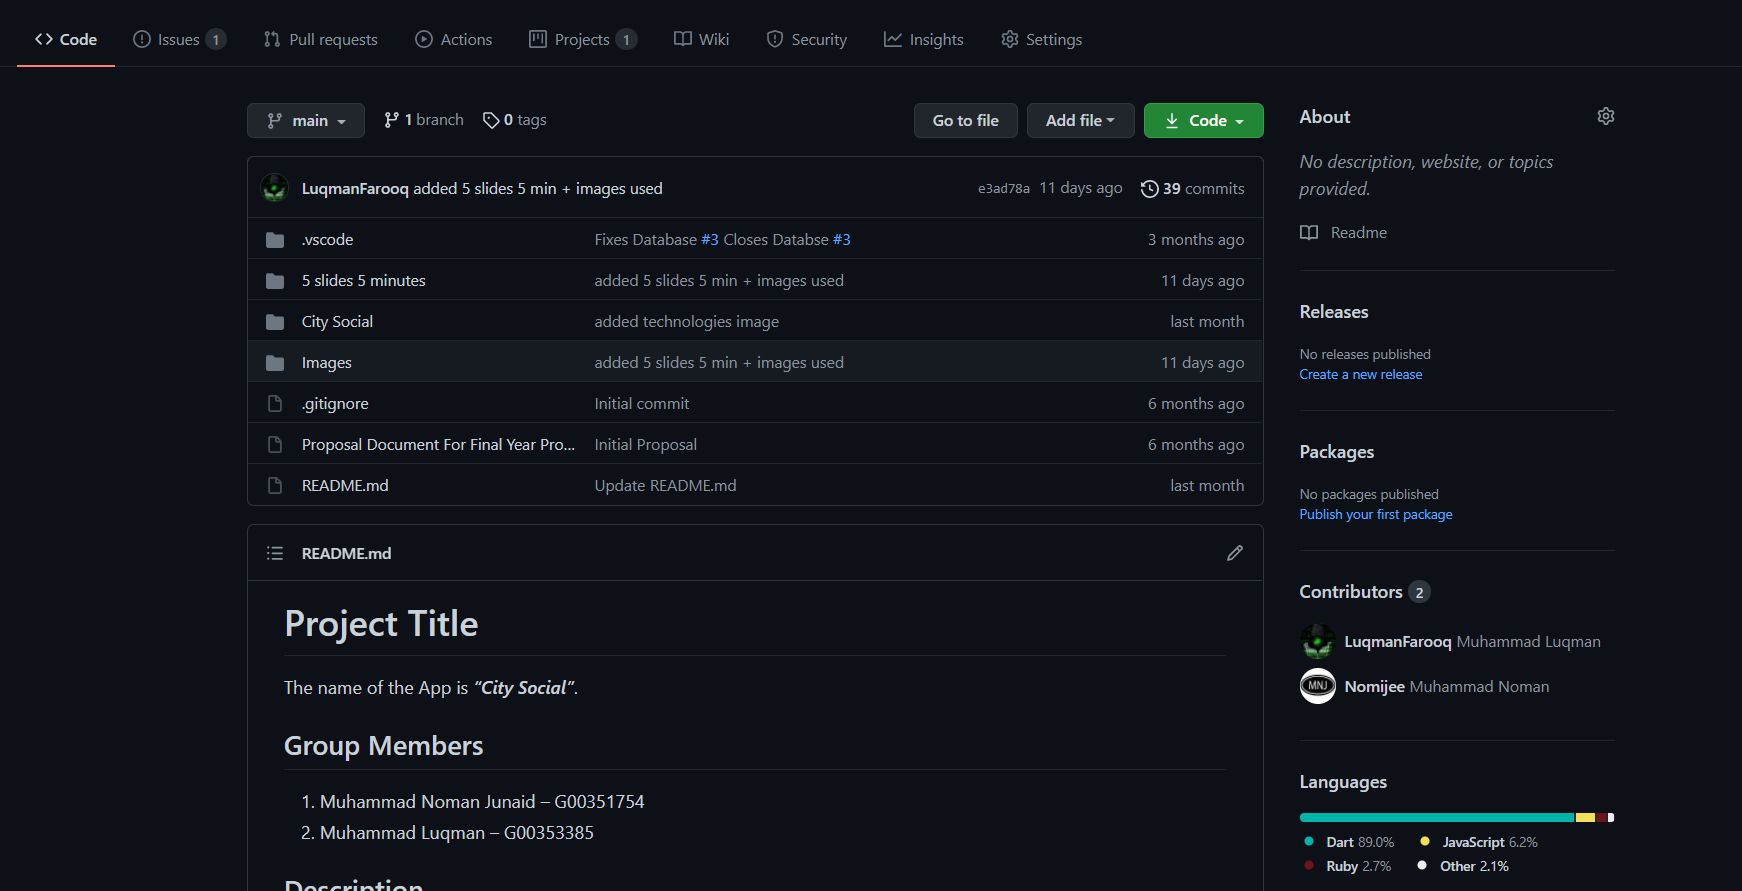
\includegraphics[scale=0.35]{img/github.PNG}
    \caption{GitHub Repository of the Project}
    \label{fig:GitHub Repository of the Project}
\end{figure}
\chapter{Methodology}
This chapter covers the various methodologies that were implemented in this project, describes the methodology that was used and how we implemented it, and also talks about how the development of the project progressed in the end. At the end of this chapter, the reader should be able to have a good impression of the scale of the project and the necessary steps that were taken throughout the project. For our final year project, we both wanted to use a constant design process to which changes and issues could be kept accounted for and so that we would be able to deal with them when they happened in an easy and dynamic way. As a result, we decided to use the Agile method would be the best fit for us as we had both had experience and knowledge of it from our previous years from the course. An Agile methodology is a certain approach to the management of a project which is greatly suited to us doing any project in Software Development. Using this method will help us to come up against any problems or difficulties such as code errors, changing the format of the project so as to suit the client's demands, etc. Agile uses work sequences that are called ‘Sprints’ which is a course of time that’s designated for certain stages in the development of a project. When creating a project, time is an important factor especially when one does Software Development so the idea of using Sprints is very important.

\section{Project Management}
\begin{figure}[!htb]
    \centering
    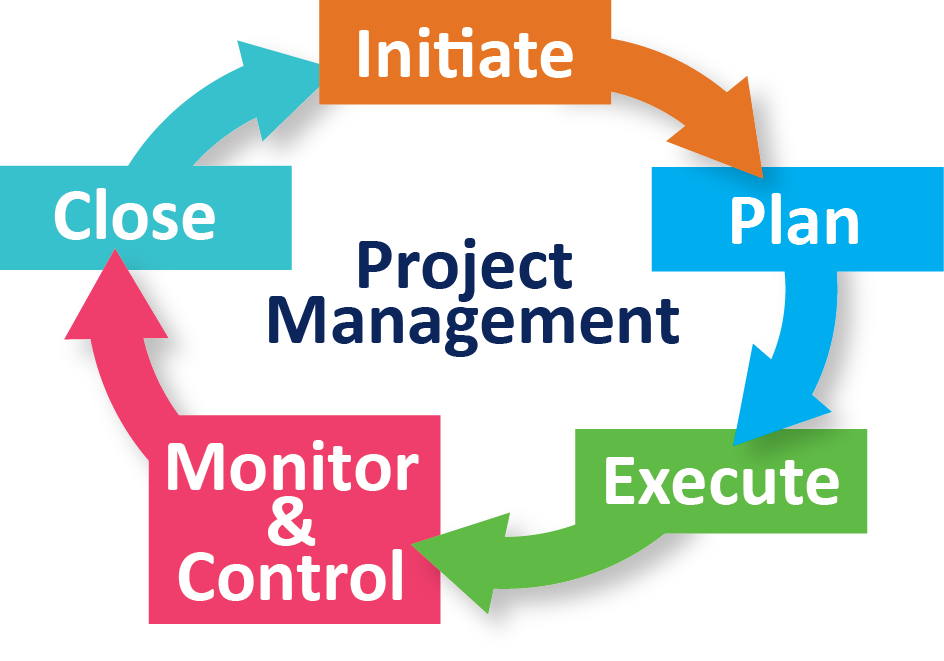
\includegraphics[scale=0.45]{img/Project Management Cycle Framework V2.png}
    \caption{Project Management Cycle Framework}
    \label{fig:Project Management Cycle Framework}
\end{figure}
Project Management is a key element of any task to ensure that the project
is laid out correctly and each component party is complete at a given date.
Because this project is a Group project we used the GitHub Kanban board to first pick features that we may want to implement and then broke them down into
separate cards that we could work on individually. This helped break down tasks
which helped in development. Project management also includes supervisor meetings and Source Control such as GitHub and Overleaf.

\subsection{Agile}
This project used Agile project management methodologies \cite{WhatisAg86:online}. An iterative approach was taken. This meant that each week we had certain tasks laid out to
be completed be that like a feature for the app. we also had short weekly/bi-weekly meetings with our supervisor where we would update him,
and asks for advice on our dissertation, app, and discussed issues that we came across while developing the app, etc.

\subsubsection{Planning and Development}
During the meeting and planning phase, the milestones and objectives for the
project were identified and broken down into simpler, and more manageable tasks. The tasks are were then grouped into sprints or iterations lasting one
to three weeks depending on the task. These are the tasks which mostly completed before each meeting with our supervisor. With each meeting, we had a task somewhat completed and we could then know the following task which we could
talk with our supervisor about beforehand. So each weekly meeting with the
supervisor started a sprint and the aim was to complete most of that sprint
before the next meeting. The plans for the project and the sprints are taken
from the User stories we created on the Kanban project and Design document.
Through this iteration, we convert the plans into working code.
\subsubsection{Design Phase}
Throughout the agile development life cycle, design is a step in every iteration/sprint. The design is gradually built on. The design is never defined at the beginning of the project. The gradual evolution of the design enables taking advantage of new technologies that come on stream as well as meeting any
new requirements brought forward by clients. The user experience is key when
designing a project/application. Every design must be user-friendly \cite{AgileSof90:online}. The type of end-user of the item must be considered when designing. This comes to play in Flutter development often as there are many different tools in development to create different features. we need to test them to know what's best for the end product e.g there are loads of icons of the came category built in a flutter that we can use have used.
\subsubsection{Testing}
Testing was carried out continuously with Visual Studio Code Emulator. Visual Studio Code has a huge amount of features the Emulator can test
a massive array of devices. So testing for this application was a continuous
process throughout every build.
\subsubsection{Unit Testing}
Every feature that was created, was tested first before integrating with the application testing was done manually by performing the operation on the developed feature and checking that does it perform the task that is expected or not. e.g saving posts to the firestore database after we press the post button the post data should be saved to the firestore which was then verified by checking the database documents that does it contains the post data which was saved for testing.
\subsection{System Integration \& Testing}
The next stage or sprint was to focus on the integration of the features and their integration testing. First, we integrated the initial project structure with the firebase. Then we starting building app features, testing them, and integrating them. we developed the sign-in page and home page of the application and then integrated and tested them together in a way that after the sign-in user is taken to the home page in this way we completed all the integration and testing. 

\subsubsection{Version Control}
Version control is the practice of tracking and managing code changes. The source code management (SCM) system provides a history of code development execution and helps resolve conflicts when merging contributions from multiple sources. For this
project, we choose Git with GitHub as our Version Control System to track our changes, log errors, and work effectively using our Agile methodology. Git is an open-source and free version control system that allows small or large projects to be stored and accessed efficiently. Features include commits, branching, staging, and workflows. GitHub allows a project to be stored remotely and for multiple people to work together seamlessly \cite{GitHub:online}.

we didn't make our own branches we just committed to the one and only master branch because we had other modules work ongoing as well so we decided to work on this project on alternate weeks e.g during week 1 Luqman will work on this project and week 2 noman will work. We didn't divide the work as front end and backend because both of us were new to these technologies so we had to do research and learn from tutorials and implement our solution and make each other understand that how our code works and what's the logic behind it so whatever feature of the app a team member developed he had to explain it to the other team member that how that works and in some cases, we research together on the same feature to be developed.

Using GitHub and Git allowed us to work simultaneously during Feb and March when we were behind the schedule and both of us had to work together at the same time on the project to increase our productivity. We also used inbuilt features on GitHub such as issue tracking. if an issue occurred or a bug was found during testing, we would make a GitHub issue, and log all our commits using the issue id. This would track our progress in fixing it and help us keep an account of the work undertaken.

\chapter{Technology Review}
This chapter discusses the different technologies used throughout the project. It discusses the advantages and disadvantages of each technology and why certain technologies were used over others. It also discusses hybrid applications compared to native applications, advantages, disadvantages, uses at different business structures, and other topics.

\section{Overview}
This Project is a Cross-platform application built with Flutter \& Dart in Visual Studio Code. Firebase is used for the database, authentication, and CRUD functionality of the app.
The following topics are discussed in detail:

\begin{itemize}
\item Flutter
\item Dart
\item Firebase
\end{itemize}

\section{Flutter}
\begin{figure}[!htb]
    \centering
    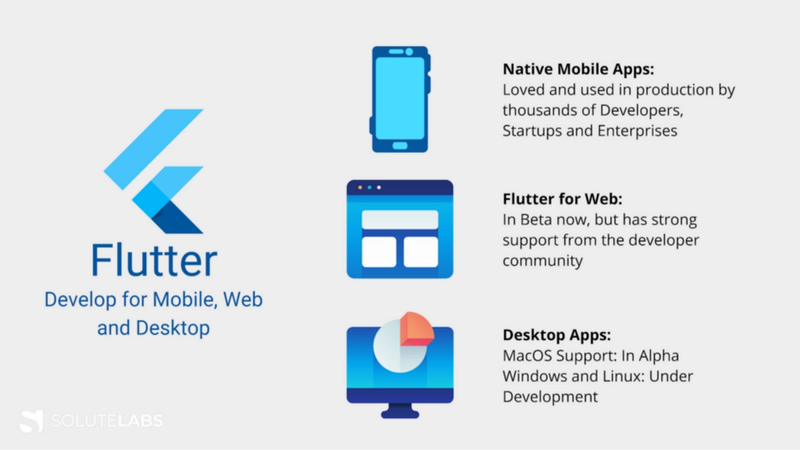
\includegraphics[scale=0.15]{img/Flutter.png}
    \caption{Flutter}
    \label{fig:Flutter}
\end{figure}
Flutter is Google's cross-platform framework that can build beautiful applications for mobile, web, and desktop using a single code base. \cite{FlutterGoogle:online}.
\subsection{how it works}
\subsubsection{Widgets}
The main idea behind Flutter is to use widgets. By combining different widgets, developers can create a complete user interface. Each of these widgets defines a structural element (such as a button or menu), a style element (font or color scheme). , Design aspects (for example, interior decoration) and many other aspects.

Flutter also provides responsive views for developers. In order to avoid performance problems when using a compiled programming language to connect to JavaScript, Flutter uses Dart. Pre-compile Dump (AOT) into native code for multiple platforms.

According to \cite{WhatisFlutter-Benefits:online} Flutter is the only mobile SDK that provides reactive views without a JavaScript bridge. This is why so many mobile developers test it in their projects.

Flutter comes with many powerful basic widgets, the following are commonly used:

Here’s a diagram of the widget tree for this UI:
\begin{figure}[!htb]
    \centering
    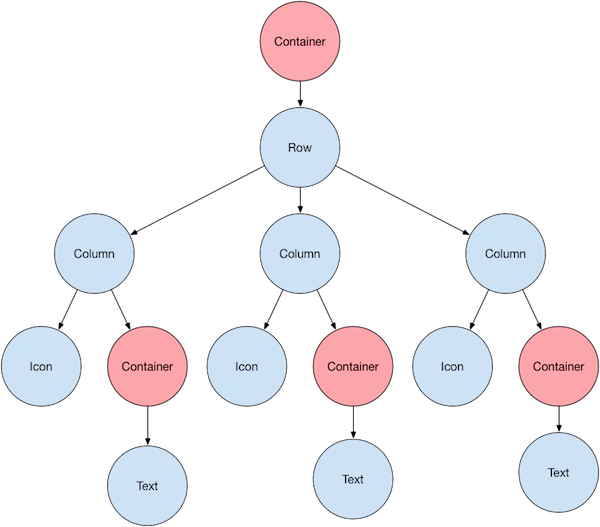
\includegraphics[scale=0.45]{img/layoutDiagramtree.png}
    \caption{Layout Diagram Tree - source - \cite{FDevLayouts:online}}
    \label{fig:Layout Diagram Tree}
\end{figure}

\subsubsection{Text}
The Text widget helps you to create a run of styled textual content inside your application \cite{widgetsFlutterDev:online}.
\subsubsection{Row, Column}
With flex widgets, we can create bendy layouts in each of the horizontal (row) and vertical (column) directions. The layout of those items is primarily based totally on the web’s flexbox format model \cite{widgetsFlutterDev:online}.
\subsubsection{Stack}
you can stack widgets in the order in which they are drawn. You can then use the widgets located on the children of the stack to position them relative to the top, right, bottom, or left side of the stack. The stack is based on an absolute design model for web page positioning \cite{widgetsFlutterDev:online}.
\subsubsection{Container}
we can use container widgets to create rectangular shapes and can decorate the container with BoxDecoration elements (such as background, frame, or shadow). The container can also have margins, padding, and limits appropriate to its size. You can use an array to convert the container into a 3D space \cite{widgetsFlutterDev:online}.
\subsection{Widget Example Code}
Here is the code that we used in our project to create the following circular progress indicator using widgets
\begin{figure}[!htb]
    \centering
    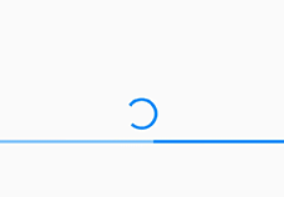
\includegraphics{img/circular progress indicator.PNG}
    \caption{Flutter Circular Progress Indicator}
    \label{fig:Flutter Circular Progress Indicator}
\end{figure}
\begin{minted}{Dart}
Container circularProgress() {
  return Container(
    // centre it in both directions horizontally and vertically
    alignment: Alignment.center,
    padding: EdgeInsets.only(top: 10.0),
    // for circular progress indicator spinning
    child: CircularProgressIndicator(
      valueColor: AlwaysStoppedAnimation(Colors.purple),
    ),
  );
}
\end{minted}

\subsection{Benefits of Flutter}
Flutter is one of the most advanced mobile applications available today. With the advantage of the development team, it is a strong competitor and will become the preferred mobile technology in the near future. \cite{WhatisFlutter-Benefits:online}. Following are the Advantages of Flutter:
\subsubsection{saves time and money}
Flutter is a cross-platform development environment. This means that software developers can use the same code base to create iOS and Android apps. Cross-platform development is the most effective way to save time and money throughout the development process.
\subsubsection{Excellent performance}
Flutter provides exceptional results for two reasons. First, it employs Dart, which compiles into native code. Second, since Flutter has its own widgets, there is no need to use OEM ones. As a consequence, contact between the app and the network is reduced. These two Flutter features ensure faster app startup times and fewer overall performance problems.
\subsubsection{Quick development thanks to hot reload}
With its hot reinstallation feature, Flutter is becoming more and more popular among mobile developers. Hot reloading allows you to view code improvements in the simulator, simulator, and hardware in real-time. In less than a second, the code changed. At the same time, the software is up and running, and developers don't have to waste time restarting it. It’s now easier to build user interfaces, add new features, and fix bugs. When an application encounters an error, you can usually fix it and continue using the application as if the error had never occurred. If you need to restart the application, you can ensure that it will be completed quickly, speeding up the development process.
\subsubsection{Compatibility}
Another advantage of Flutter is that it has its own widgets, which means fewer usability issues. Developers will encounter fewer problems with operating system versions and will spend less time testing software on earlier versions of operating systems. Ensure that its software can be used on future operating system models. When a new version of Android or iOS is released, the Flutter widgets need to be changed (because the tool does not use native platform widgets). How to update Flutter's widgets Since Google uses Flutter on a large scale internally, the Flutter team is eager to update its widget set to be as similar as possible to platform widgets. Flutter widgets can also be customized and changed by anyone. With an old version of the operating system, your application may even use new widgets!
\subsubsection{Open-source}
Flutter is an open-source application, surrounded by a group of active developers who provide help, provide complete tool documentation and create useful tools. Dart is completely free.

\subsection{Example Apps Developed with Flutter}
\begin{enumerate}
    \item Google Ads
    \item AppTree
    \item Reflectly
    \item inLapp Coffee
    \item SSHButtons
\end{enumerate}

\section{Dart}
Dart is a client-oriented programming language that can be used to build fast applications on any platform. The purpose is to provide the most powerful programming language for cross-platform development and to provide a common runtime platform for application frameworks. Customer development should give priority to the development of various build targets (Web, mobile, and desktop)  and high-quality manufacturing experience. \cite{DartDev5:online}.

\subsection{The Language}
The Dart programming language is type-safe and uses static type checking to ensure that the value of a variable always matches the static type of the variable. This is commonly referred to as "tone dialing". Although the type is required, type annotations are optional due to type inference. The dart typing scheme also has multiple uses, allowing dynamic typing to be combined with runtime checking, which is very useful when experimenting or when a lot of moving code is required. \cite{DartDev5:online}.

\begin{figure}[!htb]
    \centering
    
\includegraphics[scale=0.40]{img/dartLanguage.jpg}
    \caption{Dart Programming Language}
    \label{fig:Dart Programming Language}
\end{figure}

\subsubsection{Sample Program}
Every app has a main() function. To display text on the console, you can use the top-level print() function \cite{LanguageSampleDart:online}:
\begin{minted}{Dart}
void main() {
  print('Hello, World!');
}
\end{minted}

\subsubsection{Variables}
Even in type-safe Dart code, most variables don’t need explicit types, thanks to type inference \cite{LanguageSampleDart:online}:
\begin{minted}{Dart}
var name = 'Voyager I';
var year = 1977;
var antennaDiameter = 3.7;
var flybyObjects = ['Jupiter', 'Saturn', 'Uranus', 'Neptune'];
var image = {
  'tags': ['saturn'],
  'url': '//path/to/saturn.jpg'
};
\end{minted}

\subsubsection{Control flow statements}
Dart supports the usual control flow statements \cite{LanguageSampleDart:online}:
\begin{minted}{Dart}
if (year >= 2001) {
  print('21st century');
} else if (year >= 1901) {
  print('20th century');
}

for (var object in flybyObjects) {
  print(object);
}

for (int month = 1; month <= 12; month++) {
  print(month);
}

while (year < 2016) {
  year += 1;
}
\end{minted}

\subsubsection{Functions}
Dart Documentation recommends specifying the types of each function’s arguments and return value \cite{LanguageSampleDart:online}:

\begin{minted}{Dart}
int fibonacci(int n) {
  if (n == 0 || n == 1) return n;
  return fibonacci(n - 1) + fibonacci(n - 2);
}

var result = fibonacci(20);
\end{minted}

\subsection{Strengths \& Weaknesses of Dart}
Dart has a lot of benefits, but it also has some drawbacks:
\subsubsection{Advantages}
Dart is an open-source programming language that anyone can use for free. Google is the creator of the dart. Given that it is funded by such a large company, the language has a bright future. The dart syntax makes it easy for programmers to learn. Many complex syntactic principles of other languages have been skillfully simplified and revised by their creators. Anyone who has used C\# before can easily learn dart. The programming language was created with the Internet in mind. .Dart can be easily converted directly to JavaScript, so it can be used in modern smartphone browsers and desktop computers. All you need is a simple text editor to program in this language. However, this requires a deeper understanding of programming languages. Special editors such as Android Studio (Google) and Visual Studio Code make work easier (Microsoft).

some big advantages are below:
\subsubsection{Preemptive Scheduling}
There are many programming languages in the market, such as Java, Kotlin, Objective-C, and Swift, which tend to switch between different threads, such as B. Multiple threads run at the same time. Here, a certain period of time is allocated to each thread. In the case that the process is overwritten, the context switch will take care of that specific thread to execute the AND command. There is no locking requirement in the dart programming language because dart threads do not share a memory that can cause memory loss
\subsubsection{Garbage Collection}
Garbage collection is the reason why Google chose Dart over any other programming language, which is another key factor. Most languages require the use of locks to access certain shared resources. However, this is not the case. dart. Since Dart supports garbage collection without any errors, mobile applications developed on its platform can work normally.
\subsubsection{Single Layout Format}
Unlike other programming languages, when mobile application developers use the Dart language, there is no need to use a separate declarative layout or any type of visual interface designer. This is because the layout of the dart language is very simple and easy to read, which makes the viewing process for application developers easier. With a consistent layout, developers can easily make changes in one place and express gratitude. For all advanced dart tools, this process will save time.

\subsubsection{Disadvantages}
Dart is a programming language that is still under development. This means that the help team is not as large as JavaScript and does not have many learning tools, although this may change in the near future. Editors and their technical means on computers are known, but this is not without difficulties. Critics also pointed out that instead of trying to improve the existing language, they are bringing a new language to the market.

\section{Firebase}
Firebase is Google's web and mobile application development platform, which can be used to build, improve and extend your applications. With Firebase, developers can focus on creating a great user experience. No need to manage the server. No need to write API. Your server, API, and database are universally written, so you can customize anything that meets most needs. Firebase provides a large number of features, real-time database, cloud storage, hosting, machine learning, authentication, statistics, analysis, and more.
\begin{figure}[!htb]
    \centering
    
\includegraphics[scale=0.25]{img/firebaselogo.png}
    \caption{Firebase Logo}
    \label{fig:Firebase}
\end{figure}

\subsection{Features Used}
Firebase lets you build more powerful, secure, and scalable apps, using the world-class infrastructure. There are seven different products focused on building a better app. Our project takes advantage of Authentication, Realtime Database, and cloud functions Almost all of Firebase products are extremely useful and are worth mentioning but ill explain only those that we used. we will first summarize the products and then go into further detail on the specific products we used in our project. How the code is implemented, why we used it etc.
\subsection{Cloud Firestore}
Use NoSQL databases hosted in the cloud to store and synchronize data across users and devices worldwide. Cloud Firestore provides you with real-time synchronization and offline support as well as efficient data query. By integrating with other Firebase products, you can create true serverless applications.

we used the cloud firestore database to save all the user's data. we have collections such as Users, followers, following, posts, timeline, feed, and comments that contain the documents which are linked by their ids and contain the sub-collection in which all user information is stored.

Following is our Class model for the database that we used for our app:

\begin{minted}{Dart}
 class User {
  final String id;
  final String username;
  final String photoUrl;
  final String email;
  final String displayName;
  final String bio;

  // indicating how users are initialized
  User({
    this.id,
    this.username,
    this.photoUrl,
    this.email,
    this.displayName,
    this.bio,
  });
// factory method for deserialization of the data and is responsible for taking documents snapshot and turning into an instance of user class.
  factory User.fromDocument(DocumentSnapshot doc) {
    return User(
      id: doc['id'],
      email: doc['email'],
      username: doc['username'],
      photoUrl: doc['photoUrl'],
      displayName: doc['displayName'],
      bio: doc['bio'],
    );
  }
}
\end{minted}
Further Usage of Cloud Firestore is Explained in the System Architecture section.
\subsection{Cloud Functions}
Extend your application with customizable back-end code without having to manage and extend your own server. Firebase products, Google Cloud services, or third-party events generated through Webhooks can trigger functions.
\subsubsection{OnCreate Function}
We used the onCreate trigger of the firestore functions to listen to when followers are created and then create a timeline collection that contains 
all posts of the followed user. For this, we created a reference to the user whom we followed and select their post collection. Next, we get the following user's timeline and in the 3rd step, we fetched followed user posts and added each user's post to the following timeline. 

Below is the code for OnCreateFollower function:
\begin{minted}{Dart}
 exports.onCreateFollower = functions.firestore
.document("/followers/{userId}/userFollowers/{followerId}")
.onCreate(async(snapshot,context) => {
    // when new user is created
    console.log("Follower Created", snapshot.id);
    const userId = context.params.userId;
    const followerId = context.params.followerId;

    // step 1 is to create followed user's posts ref
    const followedUserPostsRef = admin
    .firestore()
    .collection("posts")
    .doc(userId)
    .collection('userPosts');

    // step 2 create following user's timeline ref
    const timelinePostsRef = admin
    .firestore()
    .collection('timeline')
    .doc(followerId)
    .collection('timelinePosts');

    // step 3 is to get followed user posts
    const querySnapshot = await followedUserPostsRef.get();

    // add each user's post to the following timeline
    querySnapshot.forEach(doc => {
        if(doc.exists) {
            const postId = doc.id;
            const postData = doc.data();
            timelinePostsRef.doc(postId).set(postData);
        }
    });
});
\end{minted}

Then we used this function for adding the newly created post to the timeline of each follower of the post owner.To acheive this we get all the followers of the post owner and then add the new post to each follower's timeline.Following is the code demonstration for this logic
\begin{minted}{Dart}
 exports.onCreatePost = functions.firestore
 .document('/posts/{userId}/userPosts/{postId}')
 .onCreate(async (snapshot, context) => {
    const postCreated = snapshot.data();
    const userId = context.params.userId;
    const postId = context.params.postId;

    // step 1 is to get all the followers of the user who made the post
    const userFollowersRef = admin
    .firestore()
    .collection("followers")
    .doc(userId)
    .collection('userFollowers');

    const querySnapshot = await userFollowersRef.get();

    //2nd step is to add new post to each followers timeline
    querySnapshot.forEach(doc => {
        const followerId = doc.id;

        admin
        .firestore()
        .collection('timeline')
        .doc(followerId)
        .collection('timelinePosts')
        .doc(postId)
        .set(postCreated);
    });
 });

\end{minted}
\subsubsection{OnUpdate Function}
We used the OnUpdate function of the firestore to update the timeline according to the new values when a post is updated e.g to track the like of a post.For this purpose first, we get all the followers of the post owner and update each post in each follower's timeline.

\begin{minted}{Dart}
 exports.onUpdatePost = functions.firestore
 .document('/posts/{userId}/userPosts/{postId}')
 .onUpdate(async (Change , context) => {
    const postUpdated = Change.after.data();
    const userId = context.params.userId;
    const postId = context.params.postId;

    // step 1 is to get all the followers of the user who made the post
    const userFollowersRef = admin
    .firestore()
    .collection("followers")
    .doc(userId)
    .collection('userFollowers');

    const querySnapshot = await userFollowersRef.get();

    //2nd step is to update each post in each followers timeline
    querySnapshot.forEach(doc => {
        const followerId = doc.id;

        admin
        .firestore()
        .collection('timeline')
        .doc(followerId)
        .collection('timelinePosts')
        .doc(postId)
        .get().then(doc => {
            if(doc.exists) {
                doc.ref.update(postUpdated);
            }
        });
    });
 });
\end{minted}
\subsubsection{OnDelete Function}
To delete all the user posts of the user that is unfollowed and to delete a post from all followers timeline we used the OnDelete function of the firestore.To delete all post of the unfollowed user we compare the owner id in the posts with the user id that is unfollowed and if they match we delete them.
\begin{minted}{Dart}
 // fuction that deletes all the user posts of the user that is unfollowed
 exports.onDeleteFollower = functions.firestore
 .document("/followers/{userId}/userFollowers/{followerId}")
 .onDelete(async (snapshot,context) => {
    console.log("Follower Deleted",snapshot.id);

    const userId = context.params.userId;
    const followerId = context.params.followerId;
    // deleting posts by matching the owner id in the posts with the user id that is unfollowed
    const timelinePostsRef = admin
    .firestore()
    .collection('timeline')
    .doc(followerId)
    .collection('timelinePosts')
    .where("ownerId","==",userId);

    const querySnapshot = await timelinePostsRef.get();
    querySnapshot.forEach(doc => {
        if(doc.exists) {
            doc.ref.delete();
        }
    });
 });
\end{minted}
For deleting a post from all the followers timeline which is deleted by post owner we get all the followers of the user who made the post and delete that post in each followers timeline.
\begin{minted}{Dart}
 exports.onDeletePost = functions.firestore
 .document('/posts/{userId}/userPosts/{postId}')
 .onDelete(async (snapshot,context) => {

    const userId = context.params.userId;
    const postId = context.params.postId;

    // step 1 is to get all the followers of the user who made the post
    const userFollowersRef = admin
    .firestore()
    .collection("followers")
    .doc(userId)
    .collection('userFollowers');

    const querySnapshot = await userFollowersRef.get();

    //2nd step is to delete each post in each followers timeline
    querySnapshot.forEach(doc => {
        const followerId = doc.id;

        admin
        .firestore()
        .collection('timeline')
        .doc(followerId)
        .collection('timelinePosts')
        .doc(postId)
        .get().then(doc => {
            if(doc.exists) {
                doc.ref.delete();
            }
        });
    });
 });
\end{minted}
\subsection{Authentication}
Manage your users easily and securely. Firebase Auth provides various authentication methods, including emails and passwords from external providers like Google or Facebook, and direct use of existing account systems. Create your own user interface or use our fully customizable open-source user interface.

we used firebase authentication to authenticate the app users with their google account. To do this we used the google sign in package and created a function called login which uses the google sign in the listener to check if the user signed in using their google account and to handle the sign-in we created another asynchronous function called (handleSignIn)  which check if its new user then its details such as email, name, and username are saved in the firestore and if its existing user then it's taken to the home screen.

\begin{minted}{Dart}

login() {
    googleSignIn.signIn();
  }

 handleSignIn(GoogleSignInAccount account) async {
    //if Detect when user SignIn
    if (account != null) {
      //execute the function in fireStore
      await createUserInFirestore();

      setState(() {
        isAuth = true;
      });
      //else  detect when user Signed out
    } else {
      setState(() {
        isAuth = false;
      });
    }
  }
\end{minted}
As shown Firebase is an excellent option for any developer interested in creating a mobile application, finally we will go over the Pros and Cons of choosing Firebase.

\subsection{The Pros of Firebase}
The advantages that lead to why you should choose Firebase as your app backend are as follows \cite{firebaseprosandcons:online}. 
\begin{itemize}
    \item \textbf{Databases} - Depending on your budget, Google offers robust databases to use with your apps. Both real-time and Firestore databases can be scaled in terms of size, suggesting a fully secure managed solution, that still provides you easy access to your data via the firebase console. Data updates and offline access enable the database to be used in real-time applications, and it is also possible to keep multiple databases in sync.
    \item \textbf{Wide selection of products} - Firebase provides a variety of products to make your application work properly. You can choose between real-time databases and data warehouses, store data in the cloud, and build serverless applications with integrated cloud functions.
    \item \textbf{Free to use for small developers} - The price of Firebase was initially free. This way, you can understand whether it is suitable for your application and understand all the nuances. If you have a certain amount of database storage or need a specific product, you can choose a different plan for the required product or storage. You can use the Blaze pricing calculator available on the Firebase pricing page to do this.
    \item \textbf{Good Documentation} - The entire Firebase platform is well documented. Good technical documentation, API documentation, and SDK links make all products easier to use and access. The Firebase product page contains all the information you need about integration, available platforms, manuals, and documentation. , Manual and list of supported technologies.
    \item \textbf{Accessible UI and ease of Integration} - Firebase requires minimal programming language skills and provides integration through the user interface. It is also built into Android Studio to make it easier to use. Although this eliminates the need for complex configurations, anyone can customize the application.
    \item \textbf{Google products} - Firebase's content delivery network (CDN) has been integrated into the Google Cloud Platform and integrated with all Google products. Another benefit of Google’s product is that the company is unlikely to fail or endorse the product often.
\end{itemize}

\subsection{The Cons of Firebase}
The cons of firebase are limited and depend on the scope of your project. Some of the cons are as follows \cite{Downsidefirebase:online}:
\begin{itemize}
    \item \textbf{Limited Support for Ios} - Although firebase is a cross-platform product, it focuses more on the Android mobile platform than Google products. Android Studio seamlessly integrates all Firebase products, such as test labs, authentication, etc., while iOS devices do not provide such integration.
    \item \textbf{Locked into a vendor} - Usually, this is a big problem with BaaS solutions. If the data cannot be ported to another platform, it can be considered fraud.
    \item \textbf{Unpredictable pricing} - Firebase has two price plans one is completely free which is Spark Plan and, which is perfect for newbies to Firebase. Blaze Plan is a pay-as-you-go option for large applications. This is where the problem arises-it is impossible to know in advance how the increase in traffic will ultimately affect prices. The more you spend on the product, the higher the price of Firebase. Plan; growing your business is both a blessing and a curse. Even professional Firebase integrators sometimes struggle to answer customer questions about the future cost of using Firebase.
\end{itemize}

\chapter{System Design}

\section{Chapter Introduction}
In this section, we will discuss the architecture of the application. The
components of a flutter application and how the Front-End communicates with the Back-End.

\section{System Architecture}
\begin{figure}[!htb]
    \centering
    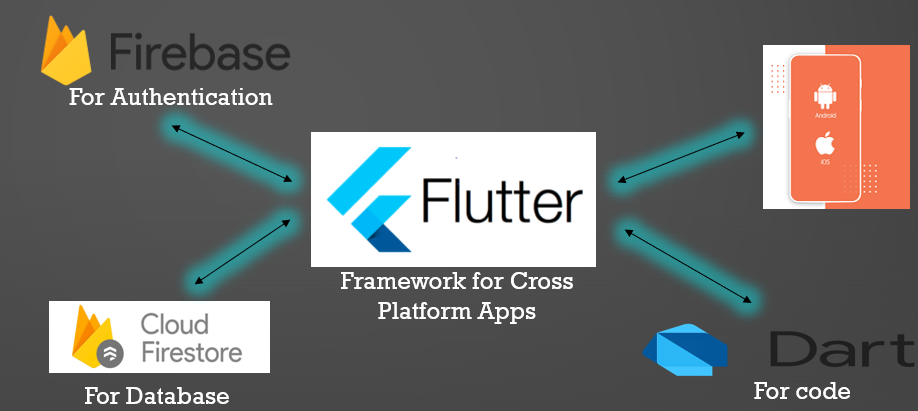
\includegraphics[scale=0.70]{img/systemArchitecture.PNG}
    \caption{System Architecture}
    \label{fig:System Architecture}
\end{figure}

\begin{itemize}
    \item \textbf{Flutter} - Platform or toolkit that is the base of our App and that we used to create the project and to implement the functionality of our project.
    \item \textbf{Dart} - Flutter only supports Dart so Dart is a programming language that we used with flutter to develop our app.
    \item \textbf{Firebase} - Firebase is a Backend-as-a-Service (Baas) that we used for the Authentication of users with google sign in.
    \item \textbf{Cloud Firestore} - This is a part of the firebase platform that we used for the Database as the database is needed for our project to store all user's data and authorized users.
\end{itemize}
\section{Project Setup}
Installed flutter from "flutter.dev", Android toolchain, and Android studio. we didn't install Vs Code as we already had it in our systems. After installing the above check-in command-line window by typing "flutter doctor" that all are the boxes are checked and no issues found in the doctor summary and finally installed an extension of flutter in Visual Studio Code. 

First created a new firebase project and named it "CitySocial" and then Created a new flutter project and added all the required assets for the project in "pubspec.yaml". 

\section{Sign In Splash Screen}
For this project, we thought to have only 1 method of login that is google login. so whenever a user visits our app they'll need to sign in and be authenticated with Google sign in order to use the app so it consists of our app title as well as a button that users can click to actually sign in. For this, we created widgets as widgets are the fundamental block of a flutter app.

\begin{figure}[!htb]
    \centering
    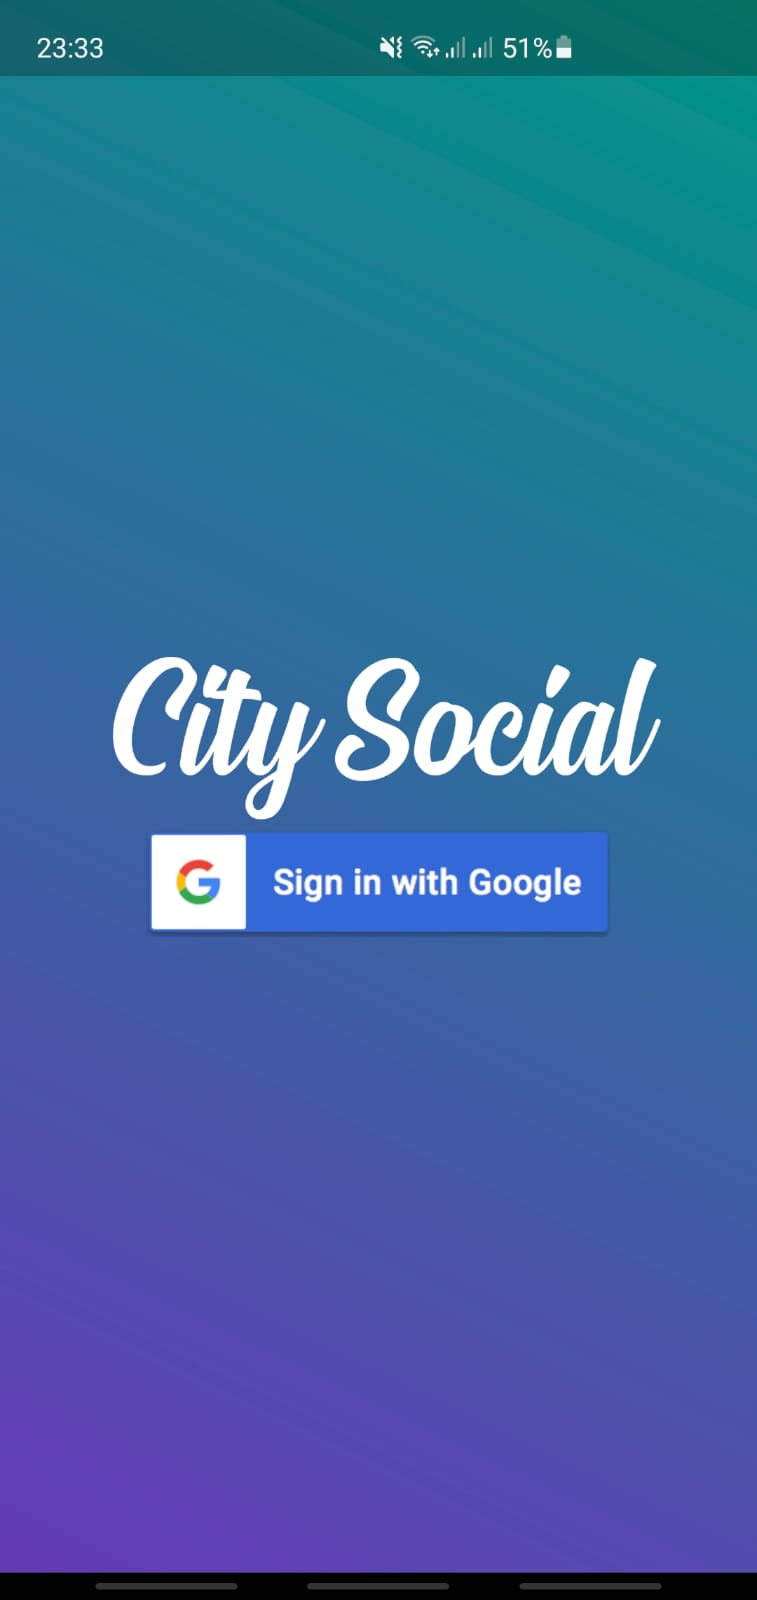
\includegraphics[scale=0.20]{AppScreenShots/SignIn Splashscreen.jpeg}
    \caption{SignIn Splash Screen}
    \label{fig:SignIn Splash Screen}
\end{figure}

The SignIn splash screen with the "SignIn with Google" button in the center is built in a widget. first, we make a scaffold for unauth screen then we make a container. the container is just a box that contains the App title "CitySocial which contains a gesture detector to detect the tap and its child is another widget with a container that contains the SignIn button image and works as the sign-in button and ontap performs the login operation. Below is the code for this Sign in screen.

\begin{minted}{Dart}
// return type of scafold widget with signin button created from signinpng image
  Scaffold buildUnAuthScreen() {
    return Scaffold(
      body: Container(
        decoration: BoxDecoration(
          gradient: LinearGradient(
            begin: Alignment.topRight,
            end: Alignment.bottomLeft,
            colors: [
              Theme.of(context).accentColor,
              Theme.of(context).primaryColor,
            ],
          ),
        ),
        alignment: Alignment.center,
        child: Column(
          mainAxisAlignment: MainAxisAlignment.center,
          crossAxisAlignment: CrossAxisAlignment.center,
          children: <Widget>[
            Text(
              'City Social',
              style: TextStyle(
                  fontFamily: "Signatra", fontSize: 90.0, color: Colors.white),
            ),
            GestureDetector(
              // checking if button works
              onTap: login,
              child: Container(
                width: 260.0,
                height: 60.0,
                decoration: BoxDecoration(
                  image: DecorationImage(
                    image: AssetImage('assets/images/google_signin_button.png'),
                    fit: BoxFit.cover,
                  ),
                ),
              ),
            )
          ],
        ),
      ),
    );
  }
\end{minted}

\subsection{Sign In}
we created a function to handle the sign-in through firebase so the function detects if the user is a new user or existing user if its a new user then it awaits for another function to be executed which shows the user a new screen to enter his/her user name which is then stored in a users collection of firestore database and the model for the database is stored in "user" file which is in a model folder in the project hierarchy and then the user is taken to the Timeline screen. if it's an existing user then it takes to the timeline screen.

here is the code responsible for the validating usernames
\begin{minted}{Dart}
@override
  Widget build(BuildContext parentContext) {
    return Scaffold(
      key: _scafoleKey,
      appBar: header(context,
          titleText: "Set up your profile", removeBackButton: true),
      body: ListView(
        children: <Widget>[
          Container(
            child: Column(
              children: <Widget>[
                Padding(
                  padding: EdgeInsets.only(top: 25.0),
                  child: Center(
                    child: Text(
                      "Create a username",
                      style: TextStyle(fontSize: 25.0),
                    ),
                  ),
                ),
                Padding(
                  padding: EdgeInsets.all(16.0),
                  child: Container(
                    child: Form(
                      key: _formKey,
                      autovalidateMode: AutovalidateMode.always,
                      child: TextFormField(
                        validator: (val) {
                          if (val.trim().length < 5 || val.isEmpty) {
                            return 'Username too short!';
                          } else if (val.trim().length > 18) {
                            return 'Username too Long!';
                          } else {
                            return null;
                          }
                        },
                        onSaved: (val) => username = val,
                        decoration: InputDecoration(
                          border: OutlineInputBorder(),
                          labelText: "Username",
                          labelStyle: TextStyle(fontSize: 15.0),
                          hintText: "Must be at least 5 characters",
                        ),
                      ),
                    ),
                  ),
                ),
                GestureDetector(
                  onTap: submit,
                  child: Container(
                    height: 50.0,
                    width: 350.0,
                    decoration: BoxDecoration(
                      color: Colors.blue,
                      borderRadius: BorderRadius.circular(7.0),
                    ),
                    child: Center(
                      child: Text(
                        "Submit",
                        style: TextStyle(
                            color: Colors.white,
                            fontSize: 15.0,
                            fontWeight: FontWeight.bold),
                      ),
                    ),
                  ),
                ),
              ],
            ),
          )
        ],
      ),
    );
  }

\end{minted}

The function below handles the signin with the google account and responsibe to switch the states between signin and not signed to the app.
\begin{minted}{Dart}
handleSignIn(GoogleSignInAccount account) async {
    //if Detect when user SignIn
    if (account != null) {
      //execute the function in fireStore
      await createUserInFirestore();

      setState(() {
        isAuth = true;
      });
      //else  detect when user Signed out
    } else {
      setState(() {
        isAuth = false;
      });
    }
  }

\end{minted}

The below function check for if the user is a new user or existing user if its a new user then it shows the user a new screen to enter his/her user name which is then stored in a users collection of firestore database and if its existing user we take him to the authenticated screen.

\begin{minted}{Dart}
createUserInFirestore() async {
 // 1) check if user exists in users collection in database (according to their id)
    final GoogleSignInAccount user = googleSignIn.currentUser;
    DocumentSnapshot doc = await usersRef.document(user.id).get();

    if (!doc.exists) {
// 2) if the user doesn't exist, then we want to take them to the create account page
      final username = await Navigator.push(
          context, MaterialPageRoute(builder: (context) => CreateAccount()));

// 3) get username from create account, use it to make new user document in users collection
      usersRef.document(user.id).setData({
        "id": user.id,
        "username": username,
        "photoUrl": user.photoUrl,
        "email": user.email,
        "displayName": user.displayName,
        "bio": "",
        "timestamp": timestamp
      });

// make new user their own follower (to include their post in their time line)
      await followersRef
          .document(user.id)
          .collection('userFollowers')
          .document(user.id)
          .setData({});

      //refetching the doc and updating
      doc = await usersRef.document(user.id).get();
    }

    currentUser = User.fromDocument(doc);
  }

\end{minted}
\subsection{Auth Screen}
The Auth screen is built with the scaffold widget whose body is a type of pageview for the scrolling timeline screen and its children contain the list of widgets which consist of the activity feed page, search user page, upload post page, and the profile page. These widgets are attached with the bottom navigation bar with their respective icons and on tapping any of the buttons its jumps to that page. Below is the code for building auth screen

\begin{minted}{Dart}
Scaffold buildAuthScreen() {
    return Scaffold(
      body: PageView(
        // building a navigation bar with buttons
        children: <Widget>[
          Timeline(currentUser: currentUser),
          ActivityFeed(),
          //pass to currentUser argument
          Upload(currentUser: currentUser),
          Search(),
          //first check current user is not null and only in that case we want id of it
          Profile(profileId: currentUser?.id),
        ],
        // adding a controller which enables us to switch between controller
        controller: pageController,
        onPageChanged: onPageChanged,
        physics:
            NeverScrollableScrollPhysics(), // because we dont want page view itself to scroll
      ),
      bottomNavigationBar: CupertinoTabBar(
        currentIndex: pageIndex,
        onTap: onTap,
        activeColor: Theme.of(context).primaryColor,
        items: [
          BottomNavigationBarItem(
            icon: Icon(Icons.whatshot),
          ),
          BottomNavigationBarItem(
            icon: Icon(Icons.notifications_active),
          ),
          BottomNavigationBarItem(
            icon: Icon(
              Icons.photo_camera,
              size: 35.0,
            ),
          ),
          BottomNavigationBarItem(
            icon: Icon(Icons.search),
          ),
          BottomNavigationBarItem(
            icon: Icon(Icons.account_circle),
          ),
        ], // providing icons so user can click on to switch page
      ),
    );
  }
\end{minted}

\section{Search Users}
The search Icon button in the bottom navigation bar takes us to the search page where we can write user names to search that user.
\subsection{SearchBar}
The search bar is created as a widget, it returns an app bar of white color with a placeholder "search a user" an account box icon at the left, and a clear icon on the right. Below is the code for this 

\begin{minted}{Dart}
 AppBar buildSearchField() {
    return AppBar(
      backgroundColor: Colors.white,
      title: TextFormField(
        controller: searchController,
        decoration: InputDecoration(
          hintText: "Search a User...",
          //togive it gray background setting filled to true
          filled: true,
          prefixIcon: Icon(
            Icons.account_box,
            size: 28.0,
          ),
          suffixIcon: IconButton(
            icon: Icon(Icons.clear),
            onPressed: clearSearch,
          ),
        ),
        onFieldSubmitted: handleSearch,
      ),
    );
  }
\end{minted}
\subsection{Search Results}
The following function returns a list of users upon search, it basically resolves our search results with the future builder so for every document it receives it deserializes it and wraps it into a text widget, and adds to the results list.

\begin{figure}[!htb]
    \centering
    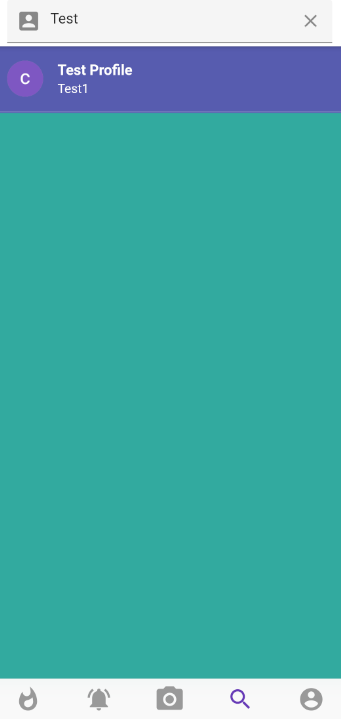
\includegraphics[scale=0.70]{AppScreenShots/searched user.PNG}
    \caption{Searched User Screenshot}
    \label{fig:Searched User Screenshot}
\end{figure}

\begin{minted}{Dart}
 buildSearchResults() {
    // we are resolving our search results feature with our future builder
    return FutureBuilder(
        future: searchResultsFuture,
        builder: (context, snapshot) {
          if (!snapshot.hasData) {
            return circularProgress();
          }
          // list of text widgets
          List<Text> searchResults = [];
          snapshot.data.documents.forEach((doc) {
            // for each user document that we get we need to deserialize it
            User user = User.fromDocument(doc);
            // wrapping into text widget and  addding the result to the searchResults list
            searchResults.add(Text(user.username));
          });
          // returning listview with its chidren being our search results
          return ListView(
            children: searchResults,
          );
        });
  }
\end{minted}

\section{Upload Post}
tap on the camera icon button on the bottom navigation bar takes to the upload screen where the user can upload an image either from the gallery or camera.
\subsection{Upload Image Button and Upload Splash Screen}
The upload image button is created as a widget whose children contain the splash  image and then its children contains a raise button specified with the shape and size of the button and its color to orange and its child as text with value "Upload Image" and all this wrapped in a container which acts as an upload splash screen.please see the code for this as follows:

\begin{figure}[!htb]
    \centering
    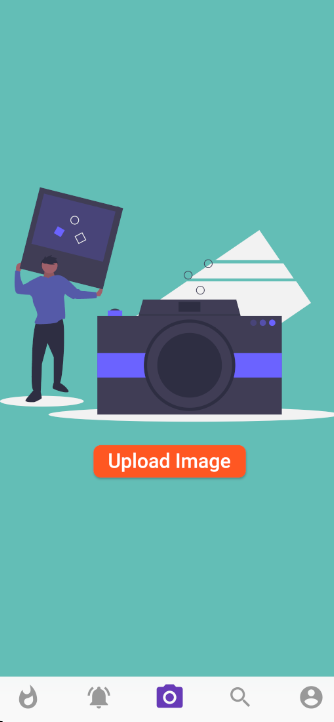
\includegraphics[scale=0.80]{AppScreenShots/upload image.PNG}
    \caption{Upload page}
    \label{fig:Upload Page}
\end{figure}

\begin{minted}{Dart}
 Container buildSplashScreen() {
    return Container(
      color: Theme.of(context).accentColor.withOpacity(0.6),
      child: Column(
        mainAxisAlignment: MainAxisAlignment.center,
        children: <Widget>[
          SvgPicture.asset('assets/images/upload.svg', height: 260.0),
          Padding(
            padding: EdgeInsets.only(top: 20.0),
            child: RaisedButton(
                shape: RoundedRectangleBorder(
                  borderRadius: BorderRadius.circular(8.0),
                ),
                child: Text(
                  "Upload Image",
                  style: TextStyle(
                    color: Colors.white,
                    fontSize: 22.0,
                  ),
                ),
                color: Colors.deepOrange,
                onPressed: () => selectImage(context)),
          ),
        ],
      ),
    );
  }

\end{minted}

\subsection{Create Post Dialog Box}
The following code creates a dialog box when the user clicks on the upload button on the upload screen and the three option to choose from, photo from camera to take and upload an image from the camera, image from the gallery to select and upload an image from gallery and cancel to exit the dialog box of upload.

\begin{figure}[!htb]
    \centering
    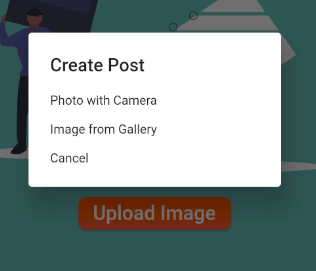
\includegraphics[scale=0.90]{AppScreenShots/create post dialog.PNG}
    \caption{Create Post Dialog Box}
    \label{fig:Create Post Dialog Box}
\end{figure}
\begin{minted}{Dart}
 selectImage(parentContext) {
    return showDialog(
        context: parentContext,
        builder: (context) {
          return SimpleDialog(
            title: Text("Create Post"),
            children: <Widget>[
              SimpleDialogOption(
                  child: Text("Photo with Camera"), onPressed: handleTakePhoto),
              SimpleDialogOption(
                  child: Text("Image from Gallery"),
                  onPressed: handleChooseFromGallery),
              SimpleDialogOption(
                child: Text("Cancel"),
                onPressed: () => Navigator.pop(context),
              )
            ],
          );
        });
  }
\end{minted}

\subsection{Upload Form}
After the image is selected from the gallery or from camera capture then it is displayed in the upload form with an arrow button at the left of the app bar to go back and the flat post button at the right of the app bar to post the image. The scaffold also contains a text box as its child with a place holder "Write a caption" on which user can write a caption and a text box with a place holder" where was this photo taken" in which a user can write a location also there is a button " use current location" to take the current location of the device and replace in the location text box above.

\begin{figure}[!htb]
    \centering
    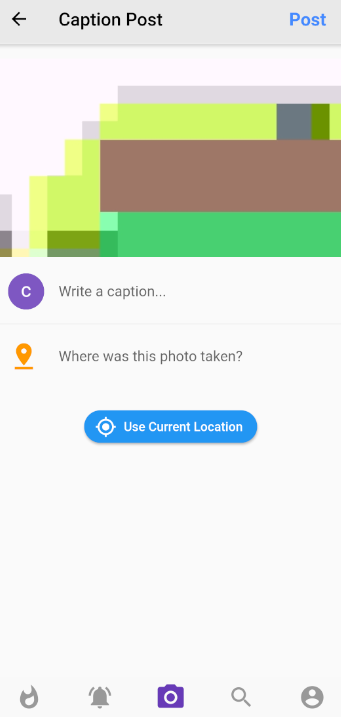
\includegraphics[scale=0.80]{AppScreenShots/caption post.PNG}
    \caption{Upload Form}
    \label{fig:Upload Form}
\end{figure}

here is the code for the above described part
\begin{minted}{Dart}
 Scaffold buildUploadForm() {
    return Scaffold(
      appBar: AppBar(
        backgroundColor: Colors.white70,
        leading: IconButton(
            icon: Icon(Icons.arrow_back, color: Colors.black),
            onPressed: clearImage),
        title: Text(
          "Caption Post",
          style: TextStyle(color: Colors.black),
        ),
        actions: [
          FlatButton(
            onPressed: isUploading ? null : () => handleSubmit(),
            child: Text(
              "Post",
              style: TextStyle(
                color: Colors.blueAccent,
                fontWeight: FontWeight.bold,
                fontSize: 20.0,
              ),
            ),
          ),
        ],
      ),
      body: ListView(
        children: <Widget>[
          //condition to show progressBar
          isUploading ? linearProgress() : Text(""),
          Container(
            height: 220.0,
            width: MediaQuery.of(context).size.width * 0.8,
            child: Center(
              child: AspectRatio(
                aspectRatio: 16 / 9,
                child: Container(
                  decoration: BoxDecoration(
                    image: DecorationImage(
                      fit: BoxFit.cover,
                      image: FileImage(file),
                    ),
                  ),
                ),
              ),
            ),
          ),
          Padding(
            padding: EdgeInsets.only(top: 10.0),
          ),
          ListTile(
            leading: CircleAvatar(
              backgroundImage:
                  CachedNetworkImageProvider(widget.currentUser.photoUrl),
            ),
            title: Container(
              width: 250.0,
              child: TextField(
                controller: captionController,
                decoration: InputDecoration(
                  hintText: "Write a caption...",
                  border: InputBorder.none,
                ),
              ),
            ),
          ),
          Divider(),
          ListTile(
            leading: Icon(
              Icons.pin_drop,
              color: Colors.orange,
              size: 35.0,
            ),
            title: Container(
              width: 250.0,
              child: TextField(
                controller: locationController,
                decoration: InputDecoration(
                  hintText: "Where was this photo taken?",
                  border: InputBorder.none,
                ),
              ),
            ),
          ),
          Container(
            width: 200.0,
            height: 100.0,
            alignment: Alignment.center,
            child: RaisedButton.icon(
              label: Text(
                "Use Current Location",
                style: TextStyle(color: Colors.white),
              ),
              shape: RoundedRectangleBorder(
                borderRadius: BorderRadius.circular(30.0),
              ),
              color: Colors.blue,
              onPressed: getUserLocation,
              icon: Icon(
                Icons.my_location,
                color: Colors.white,
              ),
            ),
          ),
        ],
      ),
    );
  }
\end{minted}
\subsection{Geo Location}
To use the geolocation we imported a package called geolocator in flutter and performed some asynchronous operations. From the geolocator class, we used the get current position method that gave the users location in latitude and longitude coordinates and placed them in the placemarks list and then in a variable we get the first element which is the 0th element of the list and extracted the locality and country information from it.
Below is the code snippet for this functionality

\begin{minted}{Dart}
 getUserLocation() async {
    Position position = await Geolocator()
        .getCurrentPosition(desiredAccuracy: LocationAccuracy.high);
    List<Placemark> palcemarks = await Geolocator()
        .placemarkFromCoordinates(position.latitude, position.longitude);
    Placemark placemark = palcemarks[0];
    String completeAddress =
        '\${placemark.subThoroughfare} \${placemark.thoroughfare}, \${placemark.subLocality} \${placemark.locality}, \${placemark.subAdministrativeArea}, \${placemark.administrativeArea} \${placemark.postalCode}, \${placemark.country}';
    print(completeAddress);
    String formattedAddress = "\${placemark.locality}, \${placemark.country}";
    locationController.text = formattedAddress;
  }
\end{minted}

\subsection{Saving to FireStore}
After the post button of the upload, the post form is pressed the then a document is stored in the "user posts" collection of the firestore which contains all the information related to a post such as postId, OwnerId, Username, mediaUrl, description, location, timestamp, and likes.

Refer to the code below for the above functionality

\begin{minted}{Dart}
 createPostInFirestore(
      {String mediaUrl, String location, String description}) {
    // to add this post to post collection
    postsRef
        .document(widget.currentUser.id)
        .collection("userPosts")
        //linking to indivisual post
        .document(postId)
        .setData({
      "postId": postId,
      "ownerId": widget.currentUser.id,
      "username": widget.currentUser.username,
      "mediaUrl": mediaUrl,
      "description": description,
      "location": location,
      "timestamp": timestamp,
      "likes": {},
    });
  }
\end{minted}

\section{Post}
The post is displayed such as they contain a header at the top with the post owners' information their avatar and user name and the location of the post. So to achieve that we used a future builder to get their data by id and return the future builder. Then the post image and underneath that it consists of a footer that consists of 3 rows one for like button and 2nd for comments and 3rd for the likes count and as well as the caption associated with the post for this we created a post model and to provide instructions for creating a post instance from a document we created a factory and also calculated the number of likes by looping over the likes map that we created in the database and checking its like value if its true we add 1

\begin{figure}[!htb]
    \centering
    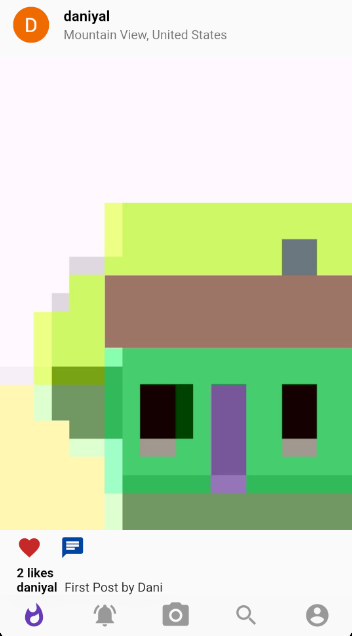
\includegraphics[scale=0.70]{AppScreenShots/Posts Structure.PNG}
    \caption{Post Structure}
    \label{fig:Post Structure}
\end{figure}

\subsubsection{Post Model factory \& likes count}

\begin{minted}{Dart}
 factory Post.fromDocument(DocumentSnapshot doc) {
    return Post(
      postId: doc['postId'],
      ownerId: doc['ownerId'],
      username: doc['username'],
      location: doc['location'],
      description: doc['description'],
      mediaUrl: doc['mediaUrl'],
      likes: doc['likes'],
    );
  }

// checking the likes map of firestore and counting the number of true values for likes
  int getLikesCount(likes) {
    // if no likes return 0
    if (likes == null) {
      return 0;
    }
    int count = 0;
    // if the key is expplicitly set to true add a like count
    likes.values.forEach((val) {
      if (val == true) {
        count += 1;
      }
    });
    return count;
  }
\end{minted}
\subsubsection{Post Header}
A post header at the top with the post owners information their avatar and user name and the location of the post.So to acheive that we used a future builder to get their data by id and return the future builder.
\begin{minted}{Dart}
 buildPostHeader() {
    // as we want to get post owners data so using future builder for that
    return FutureBuilder(
      future: usersRef.document(ownerId).get(),
      builder: (context, snapshot) {
        if (!snapshot.hasData) {
          return circularProgress();
        }
        // deserializing data
        User user = User.fromDocument(snapshot.data);
        bool isPostOwner = currentUserId == ownerId;
        return ListTile(
          leading: CircleAvatar(
            backgroundImage: CachedNetworkImageProvider(user.photoUrl),
            backgroundColor: Colors.grey,
          ),
          // if someone taps on an username we want to show their profile
          title: GestureDetector(
            onTap: () => showProfile(context, profileId: user.id),
            child: Text(
              user.username,
              style: TextStyle(
                color: Colors.black,
                fontWeight: FontWeight.bold,
              ),
            ),
          ),
          subtitle: Text(location),
          // to delete the post
          // if its the post owner t will se the icon to delete post otherwise not
          trailing: isPostOwner
              ? IconButton(
                  onPressed: () => handleDeletePost(context),
                  icon: Icon(Icons.more_vert),
                )
              : Text(""),
        );
      },
    );
  } // postheaderfunction
\end{minted}

\subsection{post footer}
Footer that consist of 3 rows one for like button and 2nd for comments and 3rd for the likes count and as well as the caption associated with the post
\begin{minted}{Dart}
 buildPostFooter() {
    return Column(
      children: <Widget>[
        Row(
          mainAxisAlignment: MainAxisAlignment.start,
          children: <Widget>[
            Padding(padding: EdgeInsets.only(top: 40.0, left: 20.0)),
            GestureDetector(
              onTap: handleLikePost,
              child: Icon(
                isLiked ? Icons.favorite : Icons.favorite_border,
                size: 28.0,
                color: Colors.red[800],
              ),
            ),
            //to separate likes and comments buttons
            Padding(padding: EdgeInsets.only(right: 20.0)),
            GestureDetector(
              //erxecute showComments function onTap
              onTap: () => showComments(
                //push to comments page
                context,
                //aruguments
                postId: postId,
                ownerId: ownerId,
                mediaUrl: mediaUrl,
              ),
              child: Icon(
                Icons.chat,
                size: 28.0,
                color: Colors.blue[900],
              ),
            ),
          ],
        ),
        Row(
          children: <Widget>[
            Container(
              margin: EdgeInsets.only(left: 20.0),
              child: Text(
                // to interpolate the number of likes
                "\$likesCount likes",
                style: TextStyle(
                  color: Colors.black,
                  fontWeight: FontWeight.bold,
                ),
              ),
            ),
          ],
        ),
        Row(
          crossAxisAlignment: CrossAxisAlignment.start,
          children: <Widget>[
            Container(
              margin: EdgeInsets.only(left: 20.0),
              child: Text(
                // to interpolate the number of likes
                "\$username  ",
                style: TextStyle(
                  color: Colors.black,
                  fontWeight: FontWeight.bold,
                ),
              ),
            ),
            // description of the user who made that post next to username
            Expanded(child: Text(description))
          ],
        ),
      ],
    );
  }
\end{minted}

\subsection{Delete Post}
The delete post is an asynchronous function that first deletes the post itself from the firebase database collection, then the post image is deleted by postId associated with the post and then all the activity feed notifications and comments are deleted.

\begin{minted}{Dart}
 //  To delete post , owner Id  and current user id must be equal, so they can be used interchangeably
  deletePost() async {
// first we delete the post itself
    postsRef
        .document(ownerId)
        .collection('userPosts')
        .document(postId)
        .get()
        .then((doc) {
      if (doc.exists) {
        doc.reference.delete();
      }
    });
    // 2nd we delete the uploaded image for the post
    // we added a child path when we created the image which was post_\$postId.jpg
    // from this post id we will be select the exact image to be deleted
    storageRef.child("post_\$postId.jpg").delete();

    // 3rd we delete all the activity feed notifications
    QuerySnapshot activityFeedSnapshot = await activityFeedRef
        .document(ownerId)
        .collection("feedItems")
        .where('postId', isEqualTo: postId)
        .getDocuments();

    activityFeedSnapshot.documents.forEach((doc) {
      if (doc.exists) {
        doc.reference.delete();
      }
    });
    // and finally deleting all comments
    QuerySnapshot commentsSnapshot = await commentsRef
        .document(postId)
        .collection("comments")
        .getDocuments();

    commentsSnapshot.documents.forEach((doc) {
      if (doc.exists) {
        doc.reference.delete();
      }
    });
  }
\end{minted}

\subsection{Like Post Heart Animation}
When a post is liked by a user then right after a click on the like button or double-tapping the photo a red heart-shaped image is displayed for 0.3 seconds.

\begin{minted}{Dart}
 buildPostImage() {
    return GestureDetector(
      //add function handleLikePost onDoubleTap
      onDoubleTap: handleLikePost,
      child: Stack(
        alignment: Alignment.center,
        children: <Widget>[
          cachedNetworkImage(mediaUrl),
          showHeart
              ? Animator(
                  duration: Duration(milliseconds: 300),
                  tween: Tween(begin: 0.8, end: 1.4),
                  curve: Curves.elasticOut,
                  cycles: 0,
                  builder: (anim) => Transform.scale(
                    scale: anim.value,
                    child: Icon(
                      Icons.favorite,
                      size: 80.0,
                      color: Colors.red,
                    ),
                  ),
                )
              : Text(""),
        ],
      ),
    );
  } // buildpostimage
\end{minted}
\subsection{Realtime Messaging with Comments}
There is a page icon beside the heat shaped like button underneath every post that when pressed takes to the comments page of that post where the user can read all comments and also post new comments. The comments are stored in the firestore collection named ``comments`` and it's linked by the post id which is then linked to another subcollection called ``comments`` and this is where the comments related to a post are stored.

To add the comment we have the reference to the comments collection and add the new comment using the ``.add`` function for firestore and specifying the post id with it.

\begin{minted}{Dart}
addComment() {
    commentsRef.document(postId).collection("comments").add({
      "username": currentUser.username,
      "comment": commentController.text,
      "timestamp": timestamp,
      "avatarUrl": currentUser.photoUrl,
      "userId": currentUser.id,
    });
\end{minted}

To display the comments we created a function to fetch the comments in realtime by using the streambuilder by referencing the postid and comments collection and then ordered the results with oldest comments at the top and we defined a comments factory model that returns the comments from its build function.
\begin{minted}{Dart}
buildComments() {
    return StreamBuilder(
        stream: commentsRef
            .document(postId)
            .collection('comments')
            .orderBy("timestamp", descending: false)
            .snapshots(),
        builder: (context, snapshot) {
          if (!snapshot.hasData) {
            return circularProgress();
          }
          List<Comment> comments = [];
          snapshot.data.documents.forEach((doc) {
            comments.add(Comment.fromDocument(doc));
          });
          return ListView(
            children: comments,
          );
        });
  }
  
  factory Comment.fromDocument(DocumentSnapshot doc) {
    return Comment(
      username: doc['username'],
      userId: doc['userId'],
      comment: doc['comment'],
      timestamp: doc['timestamp'],
      avatarUrl: doc['avatarUrl'],
    );
  }
  
  @override
  Widget build(BuildContext context) {
    return Column(
      children: <Widget>[
        ListTile(
          title: Text(comment),
          leading: CircleAvatar(
            backgroundImage: CachedNetworkImageProvider(avatarUrl),
          ),
          subtitle: Text(timeago.format(timestamp.toDate())),
        ),
        Divider(),
      ],
    );
  }
}
\end{minted}
\section{Profile page}
Tapping once at the profile icon button which is at the extreme right in the navigation bar takes to the profile page.
\begin{figure}[!htb]
    \centering
    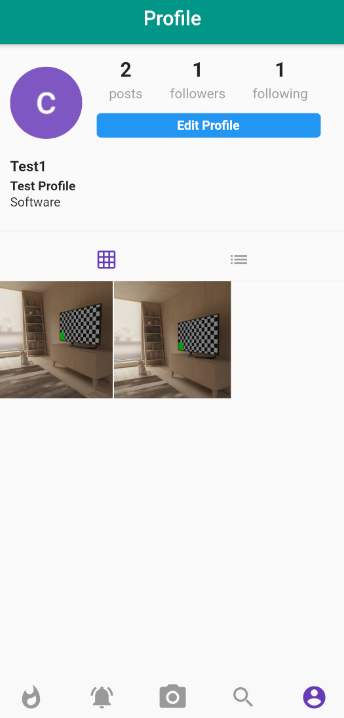
\includegraphics[scale=0.80]{AppScreenShots/profile page.PNG}
    \caption{Profile Page}
    \label{fig:Profile Page}
\end{figure}
\subsection{Profile Counts}
There is count information about the profile which includes posts count, number of followers, and number of users whom that user is following.it is achieved by building a count column widget and then getting the follower, user following, and user posts and then using the ".length" function to calculate the numbers.

\begin{minted}{Dart}
 getFollowers() async {
    QuerySnapshot snapshot = await followersRef
        .document(widget.profileId)
        .collection('userFollowers')
        .getDocuments();
    setState(() {
      followerCount = snapshot.documents.length;
    });
  }

  getFollowing() async {
    QuerySnapshot snapshot = await followingRef
        .document(widget.profileId)
        .collection('userFollowing')
        .getDocuments();
    setState(() {
      followingCount = snapshot.documents.length;
    });
  }

  getProfilePosts() async {
    setState(() {
      isLoading = true;
    });
    QuerySnapshot snapshot = await postsRef
        .document(widget.profileId)
        .collection('userPosts')
        .orderBy('timestamp', descending: true)
        .getDocuments();
    setState(() {
      isLoading = false;
      postCount = snapshot.documents.length;
      posts = snapshot.documents.map((doc) => Post.fromDocument(doc)).toList();
    });
  }
\end{minted}

\subsection{Posts Display On Profile Page}
To display the post that we fetched in the function above from the firestore database and check if the user has no posts then we show a empty splash screen and display the posts otherwise. 
\begin{minted}{Dart}
 buildProfilePosts() {
    // if we are in loading state return circular progress
    if (isLoading) {
      return circularProgress();
    }
    // if profile is empty we show empty splash screen
    else if (posts.isEmpty) {
      return Container(
        child: Column(
          mainAxisAlignment: MainAxisAlignment.center,
          children: <Widget>[
            SvgPicture.asset('assets/images/no_content.svg', height: 230.0),
            Padding(
              padding: EdgeInsets.only(top: 20.0),
              child: Text(
                "No Posts Yet!",
                style: TextStyle(
                  color: Colors.redAccent,
                  fontSize: 40.0,
                  fontWeight: FontWeight.bold,
                ),
              ),
            ),
          ],
        ),
      );
    }
    // however when we have our data
    else if (postOrientation == "grid") {
      List<GridTile> gridTiles = [];
      posts.forEach((post) {
        // serving as a child to grid tile widget
        gridTiles.add(GridTile(child: PostTile(post)));
      });
      return GridView.count(
        crossAxisCount: 3,
        childAspectRatio: 1.0,
        mainAxisSpacing: 1.5,
        crossAxisSpacing: 1.5,
        shrinkWrap: true,
        physics: NeverScrollableScrollPhysics(),
        children: gridTiles,
      );
    } else if (postOrientation == "list") {
      return Column(
        children: posts,
      );
    }
  }
\end{minted}
\subsection{ProfilePage Post orientation}
To toggle between the ListView and GridView of the post Orientation on the profile page there are two buttons below the username of the profile with two icons, an icon with grid boxes for GridView, and a sandwich icon for the ListView. User can toggle between any of them and it changes the post orientation accordingly
\begin{figure}[!htb]
    \centering
    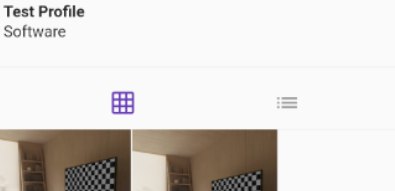
\includegraphics{img/postorient.PNG}
    \caption{Post orientation}
    \label{fig:Post orientation}
\end{figure}

\begin{minted}{Dart}
 // to togle between listview or grid view of posts
  buildTogglePostOrientation() {
    return Row(
      mainAxisAlignment: MainAxisAlignment.spaceEvenly,
      children: <Widget>[
        IconButton(
          onPressed: () => setPostOrientation("grid"),
          icon: Icon(Icons.grid_on),
          // to make the active button color using ternary opperator
          color: postOrientation == 'grid'
              ? Theme.of(context).primaryColor
              : Colors.grey,
        ),
        IconButton(
          onPressed: () => setPostOrientation("list"),
          icon: Icon(Icons.list),
          color: postOrientation == 'list'
              ? Theme.of(context).primaryColor
              : Colors.grey,
        ),
      ],
    );
  }
\end{minted}

\subsection{Edit Profile Page}
we have the Edit profile button below the profile counts on the profile page which when tapped takes the user to the edit profile form where we can update Display Name and Bio or we can log out of the account from there. To achieve this we created two-column widgets one for the Display Name and the other for the Bio.
\begin{figure}[!htb]
    \centering
    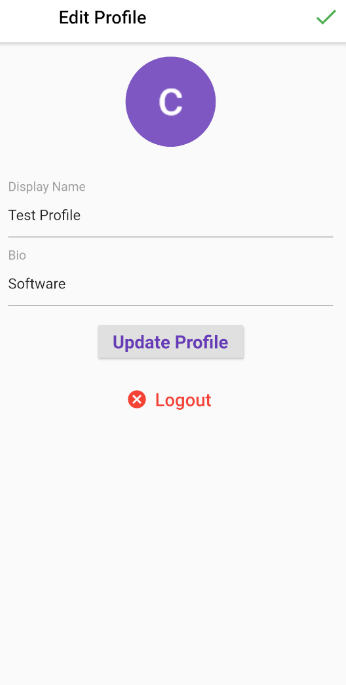
\includegraphics[scale=0.80]{AppScreenShots/edit profile.PNG}
    \caption{Edit Profile}
    \label{fig:Edit Profile}
\end{figure}
\begin{minted}{Dart}
// for creating display name field
 Column buildDisplayNameField() {
    return Column(
      crossAxisAlignment: CrossAxisAlignment.start,
      children: <Widget>[
        Padding(
            padding: EdgeInsets.only(top: 12.0),
            child: Text(
              "Display Name",
              style: TextStyle(color: Colors.grey),
            )),
        TextField(
          controller: displayNameController,
          decoration: InputDecoration(
            hintText: "Change Display Name",
            errorText: displayNameValid ? null : "Display Name too short",
          ),
        )
      ],
    );
  }
// for the bio field
  Column buildBioField() {
    return Column(
      crossAxisAlignment: CrossAxisAlignment.start,
      children: <Widget>[
        Padding(
            padding: EdgeInsets.only(top: 12.0),
            child: Text(
              "Bio",
              style: TextStyle(color: Colors.grey),
            )),
        TextField(
          controller: bioController,
          decoration: InputDecoration(
            hintText: "Change Bio",
            errorText: bioValid ? null : "Bio is too long",
          ),
        )
      ],
    );
  }
\end{minted}
Then we Validate the the data enter by the user in these field such that if name is less then 5 characters or empty then its invalid and if the the bio is greater than 100 characters then its invalid and when both are valid then we get the document of current user by id and then update the data in the database using the firestore UpdateData function.
\begin{minted}{Dart}
// conditionally set the displaynamefield and bio field
  updateProfileData() {
    setState(() {
      displayNameController.text.trim().length < 5 ||
              displayNameController.text.isEmpty
          ? displayNameValid = false
          : displayNameValid = true;
      bioController.text.trim().length > 100
          ? bioValid = false
          : bioValid = true;
    });
    // only if display name is valid and bio is valid then we will update profile data
    if (displayNameValid \&\& bioValid) {
      usersRef.document(widget.currentUserId).updateData({
        "displayName": displayNameController.text,
        "bio": bioController.text,
      });
      SnackBar snackBar =
          SnackBar(content: Text("Profile Updated Sucessfully!"));
      scaffoleKey.currentState.showSnackBar(snackBar);
    }
  }
\end{minted}
\subsubsection{logout}
To logout we use the google signout function of firebase and redirect to the SignIn page.
\begin{minted}{Dart}
// performs logout
  logout() async {
    await googleSignIn.signOut();
    // to ensure user cannt edit any more info on this page we move to home page
    Navigator.push(context, MaterialPageRoute(builder: (context) => Home()));
  }
\end{minted}
\section{Timeline}
For Timeline we have a continuous list of posts that we can scroll up and down so for that we created a timeline ref which points to the timeline collection and then in ``gettimeline()`` function we get the timeline for the current user by getting the timeline collection and we order the documents by timestamp in descending order to get the most recent post first and we save the posts in the list and iterate over it. and then call ``gettimeline`` function in the timeline widget that returns the list of posts.
\begin{figure}[!htb]
    \centering
    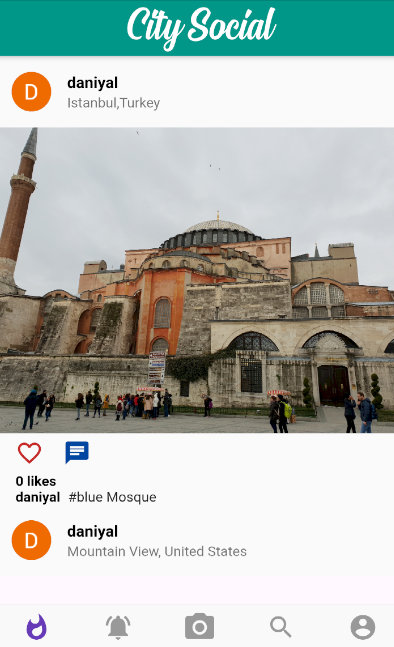
\includegraphics[scale=0.75]{AppScreenShots/timeline.PNG}
    \caption{Timeline}
    \label{fig:Timeline}
\end{figure}
\begin{minted}{Dart}
getTimeline() async {
    QuerySnapshot snapshot = await timelineRef
        .document(widget.currentUser.id)
        .collection('timelinePosts')
        .orderBy('timestamp', descending: true)
        .getDocuments();
    List<Post> posts =
        snapshot.documents.map((doc) => Post.fromDocument(doc)).toList();
    setState(() {
      this.posts = posts;
    });
  }
  
  // displays the circular widget is there are no posts and otherwise displays posts
  buildTimeline() {
    if (posts == null) {
      return circularProgress();
    } else if (posts.isEmpty) {
      return buildUsersToFollow();
    } else {
      return ListView(children: posts);
    }
  }
\end{minted}
\section{Activity Feed}
The bell icon in the bottom navigation bar is the activity feed button which when tapped takes to the activity feed where there are notifications about how started following that user, who liked that user's photo, and how commented on that user's.

For this functionality we have a collection ``feed`` in firestore database that is linked with the user ids which is linked to a subcollection named ``feedItems`` and all the notifications are stored in this collection. so to display the feed we are first storing the feed items in the firestore such as likes, comments of a post including the user who liked or commented on the post, and the timestamp when they did it for this we have an asynchronous function which has reference to the feed collection and gets the snapshot of the data that is ordered by the timestamp descending and then its added to a list that is returned by a widget.

\begin{minted}{Dart}
getActivityFeed() async {
    QuerySnapshot snapshot = await activityFeedRef
        .document(currentUser.id)
        .collection('feedItems')
        .orderBy('timestamp', descending: true)
        .limit(50)
        .getDocuments();
    List<ActivityFeedItem> feedItems = [];
    snapshot.documents.forEach((doc) {
      feedItems.add(ActivityFeedItem.fromDocument(doc));
       print('Activity Feed Item: \${doc.data}');
    });
    return feedItems;
  }
 // widget 
  @override
  Widget build(BuildContext context) {
    return Scaffold(
      backgroundColor: Colors.orange,
      appBar: header(context, titleText: "Activity Feed"),
      body: Container(
          child: FutureBuilder(
        future: getActivityFeed(),
        builder: (context, snapshot) {
          if (!snapshot.hasData) {
            return circularProgress();
          }
          return ListView(
            children: snapshot.data,
          );
        },
      )),
    );
  }
}
\end{minted}
\chapter{System Evaluation}
\section{Robust}
To make our app robust we followed the performance best practices mentioned in the flutter documentation that Accelerated the Development, Eliminated boilerplate code, and helped to build higher quality, robust app.
\subsection{Testing \& Performance}
We tested our app's robustness and performance using the Dart DevTools. it is a set of debugging and overall performance equipment for Dart and Flutter. These equipment are dispensed in IDEs such as VS Code in our case, the flutter tool, the web dev tool, and the dev tools package.

\subsubsection{Performance Test}
We started our app in profile mode. The Flutter profile mode builds and runs the application in a similar way to the release mode, but has enough advanced features to solve performance issues. To do this we just added a line of code``fluttermode:profile`` in the launch.json file of the project. Then we opened the dart dev tools and opened the performance tab of the dev tools and tested all the functionality of the app and recording the performance at the same time. 

Our app ran super smooth and responsive on the device that we deployed the app on which was "Samsung Galaxy S10". The average performance of the app was 60 FPS. As it is stated in flutter documentation \cite{PerformanceDocs:online} that ``If your frames are rendering in well under 16ms total in profile mode, you likely don’t have to worry about performance even if some performance pitfalls apply`` so considering this our overall app frame rendering was under 12ms so from this we can say that our app has no performance issues and Here is the screenshot for that below.

\begin{figure}[!htb]
    \centering
    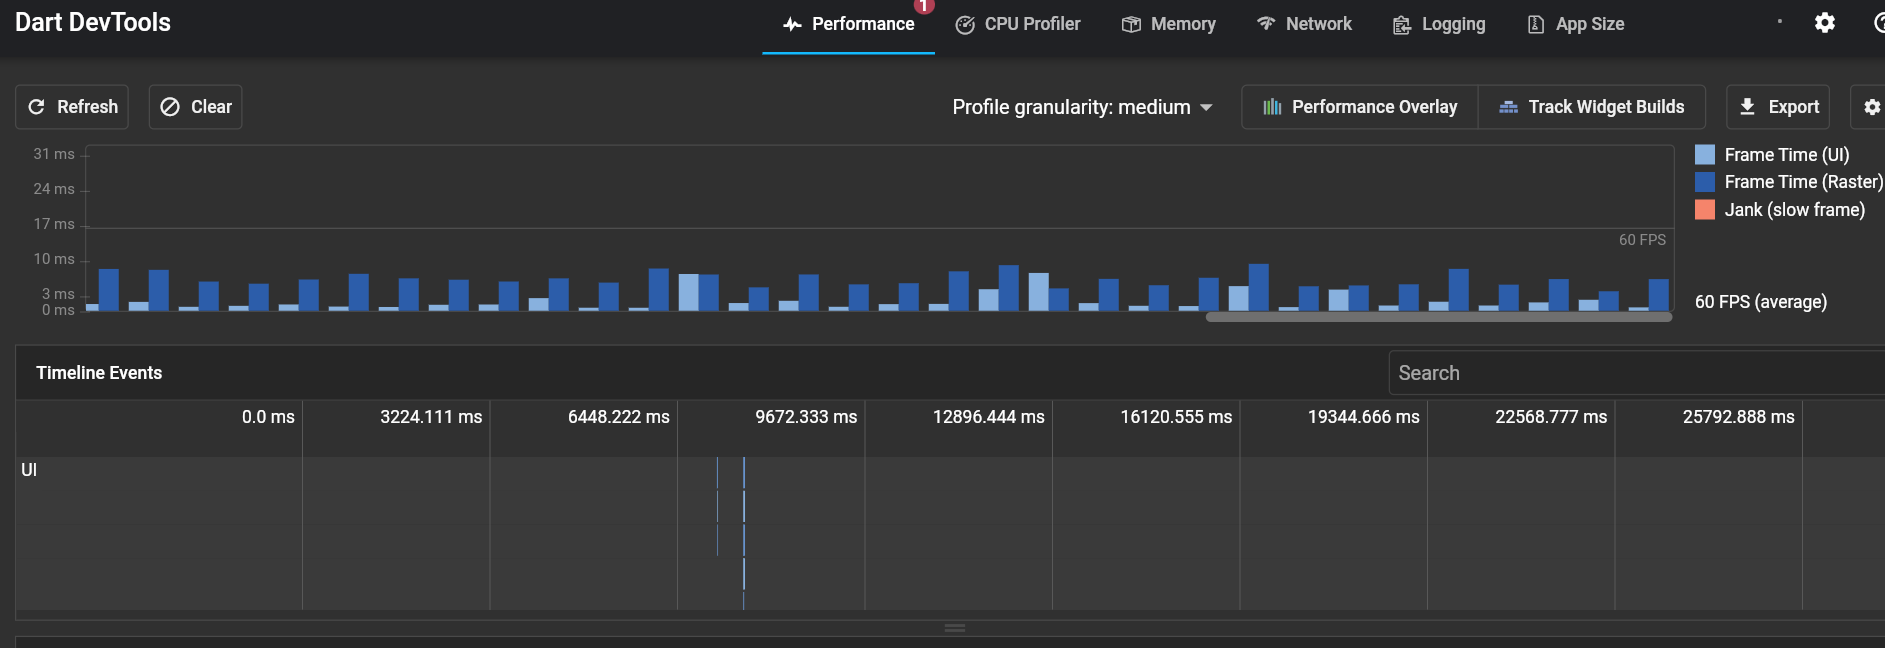
\includegraphics[scale=0.35]{img/performance test.PNG}
    \caption{Performance Test}
    \label{fig:Performance Test}
\end{figure}

\section{Evaluation of Objectives}
\subsection{Learning New Technology}
Our main goal for this project was to learn new technologies such as the Flutter framework, Dart programming language, and Firebase. As the career field that we choose is very competitive and continuously changing so for that reason to stay updated with the industry we have to learn new technologies. Through creating this project we have accomplished this goal.
\subsection{App Features}
Our goals for features were too high, although according to us we achieved around 90\% of what we wanted for this project as we couldn't implement some of the features such as Live Alerts and Push notifications, Fingerprint Authentication, Publishing App to Play store, we will talk about them in detail in the limitations \& problems section. The features that we have successfully implemented are below.
\begin{itemize}
    \item Sign in Splash Page.
    \item Sign in using google.
    \item Use of loading widgets.
    \item Search user functionality.
    \item Upload post photo using camera or gallery.
    \item Use geolocation to get the current location for photo captions.
    \item User profile.
    \item Display post count, followers count, and posts on the profile page.
    \item Display post as grid or list option on the profile page.
    \item Like post or dislike functionality with heart animation.
    \item Realtime messaging with comments.
    \item Activity feed notifications.
    \item Following or unfollowing user functionality.
    \item Displaying followed user posts on the timeline and deleting them upon
unfollowing.
    \item Suggest users to follow (i.e. new users that signup).
\end{itemize}
\subsection{Scalable and Re-Usable}
The application scales very well and functions are set with Google's recommended
standards. The application is re-usable for any type of business and implementing a new feature is extremely easy with how the application is set up.
\subsection{Responsiveness}
Our goal for the project to be responsive worked out well thanks to the development principles, Performance tips by the Flutter development team, and their great documentation that we followed. Not only is the Navigation very fast, but the read/also write from the database is almost instantaneous.

\section{Limitations and Problems we came across}
\subsection{Sign-In Error}
The First problem that we faced was that while debugging the app was the sign-in with Google feature, it was working fine in Luqman's computer but not in noman's so after researching about it we found that as Luqman created the firebase project for this app so he added SHA-1 and SHA-256 keys for his pc only so adding these keys for noman's computer and downloading the new googleservices.json file into the android/app folder of the project fixed the issue.
\subsection{Database Issue}
The second problem that we faced was that the user Data was not stored in the user's collection of the database. After researching going through our code we found that we didn't add the database model/schema so we added the database model in the user file located in the models folder. but that didn't fix the problem then we searched online for the error that we were getting and experimented with the firestore database rules after changing the rule to read|write the problem got fixed and the data stored successfully in the firestore database collection.
\subsection{Activity Feed not Displaying}
The activity feed was not displaying any notification about liking or commenting a post and following a user as well. after re-reading the code we found a simple bug that we missed calling the function in the activity feed widget that contained all the activity feed display logic so calling that function in the widget fixed the problem.
\subsection{live alerts and push notifications issue}
We implemented the live alert and push notification by linking the firebase trigger function with the activity feed so that when there is a new activity the function gets triggered and the push notification is sent to the device but for some reason, the notifications didn't work, and caused the app to crash as soon as a notification is received we couldn't figure out the reason for it and went ahead to develop rest of the features as we were short on time. But we intend to debug and fix this in the summertime.
\subsection{Fingerprint Authentication}
We implemented the fingerPrint authentication using the local\_auth dependency of flutter and created an asynchronous function to check if we are authenticated or not and if we are then move to the sign-in splash screen. But after implementation, we tested our app and the fingerprint worked and took the user to the sign-in screen and every other functionality worked but the Image upload functionality which is like the heart of our application stopped working we tried to debug it but couldn't find the cause again due to shortage of time so for that reason, we removed this functionality because it is better to have a working app with fewer functions as compared to have an app that has more functions but doesn't work properly. we intend to debug and fix this in summertime.
\subsection{Timestamp Bug}
We have used the timestamp functionality of firestore to record the time on which a comment is made and then to show it below the comments,And similarly we have this functionality to show the timestamp on activity feed page that gives notification about the user that followed us or someone like or commented on our photo.

\subsection{Publishing to play store}
As we couldn't implement all the required features as there is a saying that ``the first impression is the last impression`` so we decided not to publish the app until we have all the planned features implemented successfully and as we realized that it would cost us money on a monthly basis for using firebase functions if we publish the app and the app traffic increases and gets more requests.
\subsection{Ios limitation}
We couldn't Test the app for ios as for Ios we need Xcode for it which is not supported on windows and it required a mac for that and neither of us owns a mac and we thought it would not be feasible to buy or rent a mac for Ios implementation.

\chapter{Conclusion}

This part of our dissertation will review our project in terms of the purpose of the original intentions and examine our findings and the result of the project when we had completed it. Hopefully, by the end of reading this chapter, the reader will gain an insight into how both of us feel about the project and what we learned during the development.

\section{Context Summary}
Our final year project was the development of a Flutter Application build using Visual Studio Code, Firebase, Flutter \& Dart which was a photo-sharing social media application on which a person can socialize with other people and friends who also use this application. It has various features but the most important ones are sharing images in form of posts with caption and location using geolocation, liking and commenting on the posts of user's whom you are following or on those who follow you, having a profile with photos, name, and bio.
\section{Objectives Conclusion}
We have achieved our objectives such as learning new technologies. Although we went through the documentation of them and now have basic to intermediate knowledge about these technologies but we still need to read complete documentation of these technologies as we only used some part of these techs and to reach the advanced level of programming with these technologies we need more practice as there are famous sayings that ``practice make a man perfect and Rome was not built in a day``

we achieved another object by making the app scalable and re-usable and in summertime we have planned to add more features to it. In terms of responsiveness which was another object that we carried off successfully by making a responsive app but as we say there is always room for improvement so we will work on our further to make it more responsive.

In terms of feature implementation which was another objective we were able to implement about 90\% of the features that we planned and the rest that we mentioned above that we couldn't get working, so we intend to work on them in the summertime.

\section{opportunities identified}
we think that there is a lot of scope in expanding the application and many more features can be implemented to make the app more intuitive.
\subsection{status feature}
These days this feature is the most used one as we are social networking user our selves and everyone is using this feature every day. Basically, it displays a post (image or video) for 24 hours and the owner can also identify who saw their status. it's something similar to news headlines.
\subsection{video posts feature}
Video posing is also a very important feature these days it is similar to image posts that we have implemented but it's a video instead of images.
\subsection{Direct message (DM)}
This is a chat feature in which there is an inbox where all messages are stored and users can chat with other users who are following each other.
\subsection{Live Broadcasting}
This feature is also very popular these days due to the covid-19 pandemic. It's a kind of a video call feature but instead of one to one the video and voice is broadcasted to all followers and they all can view it and comment on it or can request to join the user that is broadcasting.

\section{Final reflections of the Project}
\begin{itemize}
    \item Using Scrum Agile Methodology helped maintain a good architecture to our development progress. We found that having a weekly meeting with our supervisor assigned to us Dr.Dominic Carr helped us keep on track on the development of the project and provided feedback on weekly meetings. We also then had our one-to-one Team meetings with each other every Monday to see how we're getting on and to see if we can fix any errors we had before our meeting every week on Wednesdays with our supervisor. However, there were still a few setbacks in these meetings as internet connection varied for some and technical issues happened at times. None the less we still were able to talk to one another at times. The Scrum Agile Methodology had been hugely helpful for us and was easy to follow.
    \item Overall the whole development of our final year project was indeed at times challenging but at the same time a worthwhile experience. Even though we both did not achieve everything we had set out at the beginning of the development as there were many aspects that were challenging as sometimes we sometimes were unable to find certain resources at time and then the lockdown being in place which limited us from working together on the project. However, still, we both attained a good insight in using Flutter while coding and insight into various technologies we used in the project. We also obtained a better bond giving each other support through the various endeavors and issues, while at the same time maintaining a positive attitude throughout the project's development even with a worldwide pandemic happening at the same time. In the end of all this with all the research, effort, and development that was put into our joint final year project, we were both happy with the end product of the project and we both were proud of ourselves as we now know it feels to work on large scale project now and will be able to work on any other future large scale projects we may have to develop in the future and we now both feel more confident as software developers now.
\end{itemize}
\chapter{Appendices}
\section{GitHub Repository}
https://github.com/LuqmanFarooq/Applied-Project-And-Minor-Dissertation

\section{Github Kanban Board}
https://github.com/LuqmanFarooq/Applied-Project-And-Minor-Dissertation/projects/1

\section{Installation Instructions}
\begin{enumerate}
    \item Navigate to the Repository and then to the ``City Social Apk`` folder in root.
    \item Download the release-apk file.
    \item copy it to any android phone.
    \item install the apk and give permission to trust app installation from unknown sources.
    \item Open and use the App.
\end{enumerate}
\printbibliography